\documentclass[final,12p,times,twocolumn]{elsarticle}


\usepackage{lineno,hyperref}
\usepackage{amsmath}

\modulolinenumbers[5]

\journal{Fluid Phase Equilibria}

\bibliographystyle{elsarticle-num}
%%%%%%%%%%%%%%%%%%%%%%%

\begin{document}
	
	\begin{frontmatter}
		
		\title{Evaluation of the SAFT-$\gamma$ Mie force field with solvation free energy calculations}% \tnoteref{mytitlenote}}
		
		\author{Isabela Q. Matos}
		\author{Charlles R. A. Abreu \corref{mycorrespondingauthor}}
		\cortext[mycorrespondingauthor]{Corresponding author}
		\ead{abreu@eq.ufrj.br}
		\address{Chemical Engineering Department, Escola de Qu\'{\i}mica, Universidade Federal do Rio de Janeiro, Av. Athos da Silveira Ramos 149, Rio de Janeiro, RJ 21941-909, Brazil}
	
		
		\begin{abstract}
   Solvation free energies can be essential in the process of evaluating and developing force fields. In addition to that, it is possible to obtain a diversity of thermodynamic informations using solvation free energies. We, at this work, studied the solvation free energy differences of molecules mimicking asphaltenes in different solvents with a coarse-grained model known as SAFT-$\gamma$ Mie force field. We obtained solvation free energies  by carrying out molecular dynamics simulations using the expanded ensemble method. The output of these simulations was then used to estimate the free energy differences. For this, we employed the MBAR method. The results with solvents other than water had low absolute deviations from experimental data. In turn, hydration free energy calculations required a binary interaction parameter estimated with output data from molecular dynamics in order to obtain accurate free energy differences. These results indicated problems on the description of the water molecule by the SAFT-$\gamma$ Mie force field, but, generally, proved that this coarse-grained model could represent the solvation free energies of the studied solute-solvent pairs.
		\end{abstract}
		
		\begin{keyword}
			solvation free energies \sep SAFT-$\gamma$ Mie 
		\end{keyword}
		
	\end{frontmatter}

	%\linenumbers
	\section{Introduction}
    Solvation free energy calculations with molecular dynamics (MD) have a variety of applications ranging from drug design in the pharmaceutical industry to the development of separation technologies in the chemical industry. {Solvation free energy is, more specifically, the difference in free energy related to the process of transferring a solute from an ideal gas phase into a liquid solution \cite{shirts2013}}. Through the study of the solvation phenomenon, it is possible to obtain information about the behavior of the solvent in different thermodynamic conditions and the influence of the solute's molecular geometry. It is also possible to calculate other important properties with the solvation free energy, namely the activity coefficient at infinite dilution, Henry constant, and partition coefficients.{ Additionally, solvation free energy calculations can be part of the methodology of calculating solubility from molecular dynamics}.
	
	The solvation free energy calculations described above are intrinsically complex due to the many competing forces interfering in the behavior of the solute-solvent interaction. In addition, free energy simulations are susceptible to sampling problems in low energy regions, and simulation results need to be correctly post-processed in order to yield free energy differences with small uncertainties. {Various simulation methodologies were developed to enable estimations of free energy differences} such as the expanded ensemble \cite{lyubartsev}, thermodynamic integration \cite{kirkwood1935}, free energy perturbation (FEP) \cite{zwanzig1954,bennet1976,mbar} and umbrella sampling \cite{TORRIE1977187}.  Utilizing  FEP methodologies, recent articles \cite{PMID:24928188,mobley2017} made available a large database of hydration free energies of small molecules using the GAFF force field. Beckstein et al. \cite{Beckstein2014} also calculated the hydration free energies for fifty-two compounds with the OPLS-AA force field. They obtained an overall root mean square deviation to the experimental data of 1.75 kcal/mol. Izairi and Kamberaj \cite{izairi2017} studied hydration free energies but with the intention of comparing the polar and nonpolar contributions. Garrido et al. \cite{garrido,garrido2011} calculated the free energy of solvation of large alkanes in 1-octanol and water with three different force fields (TraPPE, GROMOS, and OPLS-AA/TraPPE). These authors also estimated the solvation free energy of propane and benzene in non-aqueous solvents like n-hexadecane, n-hexane, ethylbenzene, and acetone with the TraPPE-UA and TraPPE-AA force fields. Roy et al. \cite{roy2017}  addressed the choice of the Lennard-Jones parameters for predicting solvation free energy of different solutes in 1-octanol. They calculated the solvation free energy of a set of 205 small organic molecules in 1-octanol and found that the force field parametrization of n-octanol proposed by  Kobryn and Kovalenko \cite{doi:10.1063/1.2972978} provided the best agreement to the experimental data. Gon\c{c}alves and
	Stassen  \cite{goncalves} calculated the free energy of solvation using the polarizable continuum model coupled to molecular dynamics simulation with the GROMOS force field. These calculations were done with a representative set of solutes and with the solvents tetrachloride, chloroform, and benzene. Using the GAFF and the polarizable AMOEBA force fields, Mohamed et al.  \cite{mohamed2016} evaluated the solvation free energy of small molecules in toluene, chloroform, and acetonitrile, and obtained a mean unsigned error of 1.22 kcal/mol for AMOEBA and 0.66 kcal/mol for GAFF. To define the role of solvent water in the docking structure determination of proteins, Matubayasi  \cite{MATUBAYASI201745} developed a method to compute the solvation free energy of proteins while using OPLS-AA force field for the solutes and TIP3P for water. Genheden \cite{doi:10.1021/acs.jctc.5b00963} expanded the ELBA force field to calculate solvation free energies of more than 150 solutes taken from the Minnesota solvation
	database in polar (water, hexanol, octanol, and nonanol) and apolar (hexane, octane, and nonane) solvents. He obtained mean absolute deviations of 1 kcal/mol for water and 1.5 kcal/mol for hexane. In this model, three carbons are represented by a single bead and water is also represented by a single bead. 	

	As can be seen in the previous paragraph, solvation free energy simulation is performed in the literature using a variety of force field since the choice of force field can be another influencing factor in the output of these calculations. Hence, we, in this study, assess the efficiencies and shortcomings of the SAFT-$\gamma$ Mie coarse-grained force field  \cite{avendano2011} with solvation free energy calculations for a variety of pairs solute-solvent. We chose a coarse-grained force field because these kind of models generally reproduce free energy differences since the effects of reducing degrees of freedom in the entropy are counterbalanced by the reduction of enthalpic terms \cite{kmiecik2016}. This fact makes these models a viable option to decrease the computational time of solvation free energy calculations. Additionally, deficiencies in the description of small molecules by coarse-grained models can be revealed by free energy calculations \cite{mobley2007,shirts2013}. We specifically picked  the SAFT-$\gamma$ Mie force field because it uses, unlike the majority of the force fields, the Mie potential \cite{MIE} and because its method of obtaining parameters is more straightforward than those of other models. It was initially parameterized with pure component equilibrium and interfacial tension data \cite{avendano2011}, and this strategy has provided satisfactory results. Examples include the prediction of phase equilibrium of aromatic compounds \cite{muller2017}, alkanes, light gases \cite{herdes2015}, and water \cite{lobanova2015}, thermodynamic properties of carbon dioxide and methane \cite{cassiano1}, multiphase equilibrium of mixtures of water, carbon dioxide, and n-alkanes \cite{lobanova2016}, and water/oil interfacial tension \cite{herdes2017}.

	We selected the solvents and solutes in our free energy calculations with the intention of testing the force field with standard sets used as a benchmark in solvation free energy calculations and with polycyclic aromatic substances used as models to asphaltenes. Asphaltenes are complicated to characterize by determining their composition on a molecular basis, but the literature broadly accepts that they can be described as a fraction of crude oil soluble in toluene and insoluble in n-alkanes (pentane, hexane, heptane) \cite{SJOBLOM2003399}. They have motivated many studies with interest in developing models for their structure and behavior due to all the problems they can cause during their transportation and refining such as precipitation during the oil processing \cite{SJOBLOM20151}. This precipitation issue is a recurrent problem due to the growing market of the production of crude oil in deep waters, whose conditions are favorable to precipitation \cite{AIC:AIC10243}. As an example, asphaltene precipitation due to pressure drop can clog oil production equipment and cause a growth in the cost of production \cite{doi:10.1021/ef010047l}. All these factors make the understanding of the behavior of asphaltenes in different chemical and physical environments relevant to the oil industry. As we said, asphaltene characterization still faces some issues. Hence, we choose to use polycyclic aromatic hydrocarbons (PAHs), which have well-defined characteristics, to initially test the efficiency of the SAFT-$\gamma$ Mie force field in describing the solvation phenomenon. PAHs are a group of organic compounds that have fused rings, carbon and hydrogen in their structure \cite{RAVINDRA20082895}. The ones utilized in this work were phenanthrene, anthracene, and pyrene since they share similarities with asphaltenes regarding their solubility. In this context,  we selected compounds that are used to characterize asphaltenes (toluene, hexane) as solvents in our free energy calculations. We also tested the anti-solvent/solvent effect of carbon dioxide due to its influence in asphaltene precipitation during the oil processing \cite{SOROUSH2014405}. With these calculations of solvation free energies with the SAFT-$\gamma$ Mie model, we intend to improve this force field and provide satisfactory solvation free energy estimates of PAHs with a coarse-grained model. The success of the description of small asphaltene-like compounds by this force field can then open up the possibility of obtaining satisfactory results for more complex asphaltene models with a force field with a low computational cost.
	
	
	

	\section{Computational Methods}
	
	\subsection{SAFT-$\gamma$ Mie Force Field}
	
	The SAFT-$\gamma$ Mie force field uses a top-down coarse-graining methodology in its parameterization. This methodology aims to obtain the intermolecular parameters from macroscopic experimental data such as fluid-phase equilibrium or interfacial tension data. The idea is that the force field parameters estimated with the SAFT-VR Mie EoS can be used in molecular simulations since both the equation of state and the force field use the same explicit intermolecular potential model (Mie potential):
	
	\begin{equation}
	\begin{aligned}
	U_{Mie}(r) {}=& \epsilon\frac{\lambda_r}{\lambda_r - \lambda_a} \left(\frac{\lambda_r}{\lambda_a} \right)^{\left( \frac{\lambda_a}{\lambda_r - \lambda_a} \right)}  \left[ \left(\frac{\sigma}{r} \right)^{\lambda_r} - \left(\frac{\sigma}{r} \right)^{\lambda_a} \right].
	\end{aligned}
	\label{eqn:miepotential}
	\end{equation}
	
	The parameter $\epsilon$ is the potential well depth, $\sigma$ is the segment diameter, r is the distance between the spherical segments, $\lambda_r$ is the repulsive exponent and $\lambda_a$ is the attractive exponent. This force field has the advantage of incorporating the degrees of freedom provided by the use of the Mie Potential \cite{herdes2015}. This flexibility offers the exploration of a vast parameter space without using an iterative simulation scheme \cite{avendano2011}. Despite these advantages, the force field can be restricted by the shortcomings of the equation of state. As an example, the lack of an association term in the equation can cause an inadequate representation of the properties of hydrogen bonding compounds.
	
	Each substance has initially five parameters to be estimated ($m_s,\ \sigma,\ \epsilon,\ \lambda_{r},$ and, $ \lambda_{a}$) according to Eq. \ref{eqn:miepotential}. The number of segments is usually fixed in an integer value since each segment represents one pseudo-atom. The attractive parameter is generally fixed due to its high correlation with the repulsive parameter. Usually, the chosen value for this parameter is 6, corresponding to the London model, which is a good representation of the dispersion scale of most simple fluids that do not have strong polar interactions \cite{ramrattan2015,herdes2015}.  There are two strategies to obtain these parameters: one is by fitting the SAFT-VR Mie EoS to experimental data such as vapor pressure and liquid density \cite{avendano2013}, and the other one is by using corresponding states parametrization \cite{mejia2014}. Here, the first strategy was used to find the parameters for phenanthrene with vapor-liquid equilibrium data \cite{murphy,osborn} following the methodology proposed by M\"{u}ller and Mej\'{\i}a \cite{muller2017}.  The parameterization was carried out with the number of segments equal to five and with a geometry such as that in Figure \ref{fig:fen5}, since this level of coarse-graining was also used for a similar molecule (anthracene) in the original paper.
	\begin{figure}[th]
		\centering
		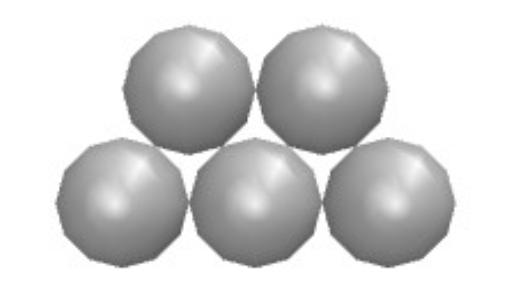
\includegraphics[width=0.25\textwidth]{Figures/fen5}
		\caption{Representation of phenanthrene with the geometry proposed by M\"{u}ller and Mej\'{\i}a \cite{muller2017}.}
		\label{fig:fen5}
	\end{figure}
	
	The parameters for the other compounds were retrieved from the literature, and all these parameters are exposed in Table \ref{tbl:parameters}. For a mixture, the mixing rules used can be seen in Eqs. \ref{eqn:sigmamix} to \ref{eqn:epsmix} \cite{lafitte2013} .
	
	\begin{equation}
	\sigma_{ij} =\frac{\sigma{ii}+\sigma{jj}}{2},
	\label{eqn:sigmamix}
	\end{equation}
	\begin{equation}
	\lambda_{k,ij} -3 =\sqrt{(\lambda_{k,ii}-3)(\lambda_{k,jj}-3)}, \quad k=r,a,
	\label{eqn:lambdamix}
	\end{equation}
	\begin{equation}
	\label{eqn:epsmix}
	\epsilon_{ij} =(1-k_{ij})\frac{\sqrt{\sigma_{ii}^{3}\sigma_{jj}^{3}}}{\sigma_{ij}^{3}}\sqrt{\epsilon_{ii}\epsilon_{jj}},
	\end{equation}

   The $k_{ij}$ is a binary interaction parameter to correct the deviations of the mixing rule for chemically distinct compounds that can be fitted to experimental or molecular simulation data. This necessity of an additional parameter raises the question of the quality of these mixing rules and make us wonder if new mixing rules could be used to describe the mixing potential well parameter. Since these were the available mixing rules and the ones employed by other papers that used this force field, we ended up using Eqs. \ref{eqn:sigmamix} to \ref{eqn:epsmix} in our study. However, the binary interaction parameter was only necessary for aqueous mixtures in our study.  
	
	\begin{table}[h]
		\centering
		\caption{SAFT-$\gamma$ Mie Force Field for each substance used in this work.}
		\label{tbl:parameters}
		\begin{tabular}{ccccc}
			\hline\hline
			& $m_s$ & $\epsilon/\kappa_{b}$ (K) & $\sigma (\dot{A})$ & $\lambda_r$ \\ \hline
			Water \cite{lobanova2016}        & 1     & 305.21               & 2.902              & 8.0         \\
			Propane \cite{herdes2015}        & 1     & 426.08               & 4.871              & 34.29       \\
			Carbon dioxide \cite{herdes2015} & 2     & 194.94               & 2.848              & 14.65       \\
			Hexane \cite{herdes2015}         & 2     & 376.35               & 4.508              & 19.57       \\
			Octanol \cite{ervik2016}         & 3     & 495.71               & 4.341              & 28.79       \\
			Toluene \cite{muller2017}        & 3     & 268.24               & 3.685              & 11.80       \\
			Benzene \cite{muller2017}        & 3     & 230.30               & 3.441              & 10.45       \\
			Pyrene \cite{muller2017}         & 4     & 459.04               & 4.134              & 15.79       \\
			Anthracene \cite{muller2017}     & 5     & 259.68               & 3.631              & 9.55        \\
			Phenanthrene                     & 5     & 262.74               & 4.077              & 9.55        \\ \hline\hline
		\end{tabular}
		
	\end{table}
	
	\subsection{Expanded Ensemble}
	
	The strategy chosen in this work to calculate the solvation free energy differences  was to use an alchemical method in which the solute molecule is gradually inserted in the solvent using a  thermodynamic path \cite{klimovich}. Each insertion or alchemical state is represented by a coupling parameter, $\lambda$, that ranges from 0 to 1. When $\lambda=0$, there is no interaction with the solvent and, when $\lambda=1$, the interactions are fully activated. Since the force field used does not explicitly take in consideration  the charges, the interactions are only due to the Mie potential. For the coupling of the Mie Potential, we propose generalized softcore Mie potential based on the softcore potential of Beutler et al.  \cite{beutler} :
	\begin{equation}
	\label{eq:miesoftcore}
	\begin{aligned}
	U_{Mie}^{sc}(r) {}=& \lambda\epsilon\frac{\lambda_r}{\lambda_r - \lambda_a} \left(\frac{\lambda_r}{\lambda_a} \right)^{\left( \frac{\lambda_a}{\lambda_r - \lambda_a} \right)} \cdot \\ 
	&  \left\lbrace\frac{1}{\left[\alpha(1-\lambda)+ (r/\sigma)^{\lambda_a}\right]^{\lambda_{r}/\lambda_{a}}}  \mathrm -  \right. \left. \frac{1}{\alpha(1-\lambda)+(r/\sigma)^{\lambda_a}}\right\rbrace .
	\end{aligned}
	\end{equation}
	where $\alpha$ is a constant whose value is  normally assumed to be 0.5. We decided to use the Expanded Ensemble method \cite{lyubartsev} in our solvation free energy simulations since it allows a non-Boltzmann sampling scheme of different states in a single simulation. In this scheme, the sampling is done by biasing the phase space exploration process with weights not related to the statistical ensemble. The partition function of the statistical expanded ensemble, $Z^{EE}$, is obtained from the probability distributions corresponding to each $\lambda$. Hence, $Z^{EE}$ is defined as a sum of subensembles $Z_{i}$ in different values of $\lambda$, that is,
	
	\begin{equation}
	Z = \sum_{i=1}^{N} Z_{i} exp(\eta_{i}),
	\label{ee}
	\end{equation}   
	where N is the number of alchemical states, $\eta_{i}$ is the arbitrary weight of the subensemble at each state, and $Z_{i}$ is the configurational partition function of state i. Here, we followed the flat-histogram approach \cite{bernd1992,bernd1993,dayal2004} to calculate the weights. This strategy aims to obtain adequate sampling by ensuring that all the states have an equal number of visits, i.e. the ratio of the probability of sampling state i ($\pi_{i}$) to the probability of sampling state $j$ ($\pi_{j}$) is equal to one. Using this relation, the following equation can be obtained:
	
	\begin{equation}
	\label{eqn:weight}
	(\eta_{i} - \eta_{j})_{k+1} = \beta(G_i-G_j)_{k} .
	\end{equation}
	
	Eq. \ref{eqn:weight} proposes that the choice of weights is dependent on the free energies that we are attempting to obtain. This equation is then solved iteratively with trial simulations. For the first simulation, the values of $\eta$ are set to zero, and the histogram of the states visited is obtained. With this histogram, it is possible to estimate the free energy differences and, since the weights are related to the free energies by Eq. \ref{eqn:weight}, the next values of $\eta$ can be calculated. This iteration goes on until a uniform distribution is attained. The weights found are then used in a longer simulation to obtain the final solvation free energies. The choice of the $\lambda$ set corresponding to overlapping alchemical states are crucial to acquire accurate free energy differences. In this work, the method chosen to obtain the optimal staging of the $\lambda$ domain is the one developed by Escobedo and Martinez-Veracoechea  \cite{escobedo2007} with a basis in the study of  Katzgraber et al \cite{1742-5468-2006-03-P03018}. This method targets "bottlenecks" in the simulation. It does that by optimizing $\lambda$ through the minimization of the number of round trips per CPU time between the lowest ($0$) and highest ($1$) values of $\lambda$. The optimization is specifically done by maximizing the steady-state stream $\phi$ of the simulation, which "walks" among the values of $\lambda$. This flow is estimated from a Fick's diffusion type of law:
	
	\begin{equation}
	\phi = D(\Lambda) \Pi (\Lambda) \dfrac{dx(\Lambda)}{d \Lambda}.
	\label{eqn:stream}
	\end{equation}
	
	In the equation above, $\Lambda$ is the actual continuous value of the coupling parameter. This continuous function of $\lambda 's$ is obtained by interpolating the $\lambda$ set linearly. $D(\Lambda)$ is the diffusivity at  state $\Lambda$ and $x(\Lambda)$ is the fraction of times that the trial simulation at state $\Lambda_{i}$ has most recently visited the state $\lambda=1$ as opposed to state $\lambda=0$. The derivative ${dx(\Lambda)}/{d \Lambda}$ is approximated with the central finite differences method. Finally, $\Pi (\Lambda)$ is the probability of visiting $\Lambda$:

	\begin{equation}
	\Pi (\Lambda) = \dfrac{C^{'} \bar{\Pi} (\lambda)}{\Lambda_{i+1} - \Lambda_{i}}.
	\label{eqn:plambda}
	\end{equation}
	
	The $C^{'} $ term in the equation above represents a constant and $\bar{\Pi} (\lambda)$ is the arithmetic average of the frequency of visits to the $\Lambda$ state:
	
	\begin{equation}
	\bar{\Pi}_{i} (\lambda) = \dfrac{\pi_{i+1} - \pi_{i}}{2}.
	\label{eqn:barplambda}
	\end{equation}
	
	The $\phi$ is maximum when the optimal probability $\Pi^{'}(\Lambda_{i})$ of visiting state $\Lambda_{i}$ is proportional to $1/\sqrt{D(\Lambda)}$ \cite{trebst2004}. With that information, it is possible to estimate the diffusivity using one trial simulation with the following equation:
	
	\begin{equation}
	D(\Lambda) = \dfrac{\Lambda_{i+1} - \Lambda_{i}}{\bar{\Pi} (\lambda) {dx(\Lambda)}/{d \Lambda}}.
	\label{eqn:diff}
	\end{equation}
	
	Hence, we can calculate $\bar{\Pi} $ and, consequently, the cumulative probability, which is used to obtain the new $\lambda$ state, by
	
	\begin{equation}
	\Phi = \int_{\lambda =0}^{\lambda =1} \Pi^{'}(\Lambda_{i}) d \Lambda = \dfrac{i}{K},
	\label{eqn:cumfun}
	\end{equation}
	where $K$ is the total number of $\lambda$ states. In order to carry out our solvation free energy simulations, we obtained these cumulative probabilities for every $\lambda$ set we estimated. A graphical demonstration of the relation between the optimized coupling parameters and the cumulative probability of Eq. \ref{eqn:cumfun} is presented in our results in Figure \ref{fig:optimized_cdf}.

	\section{Molecular Dynamics Simulations}\label{mds}
	
	
	Using the parameters of Table \ref{tbl:parameters}, we carried out molecular dynamics simulations to estimate solvation free energy differences. The chosen software package to perform the simulations was LAMMPS  \cite{lammps}. In this package, the equations of motion were integrated with the velocity-Verlet algorithm \cite{verlet} with a time step of 2 fs. As required by the coarse-grained model,  molecules with more than one bead were treated as rigid bodies. The thermostat and the barostat were the Nos\'{e}-Hoover chains as described in Hoover \cite{PhysRevA.31.1695} and Martyna et al.  \cite{doi:10.1063/1.463940} with damping factors of 100 and 1000 time steps, respectively. For the rigid bodies in our simulations, we used the rigid-body algorithm of Kamberaj et al \cite{kamberaj}. Electrostatics interactions are not explicitly accounted for by the SAFT-$\gamma$ Mie force field. Hence, we did not compute Coulombic interactions. The potential cutoff was equal to 20 \AA $\,$ \cite{muller2017} with a neighbor list skin of 2 \AA. The initial configurations of the solvated systems were also generated using the Playmol package, which is integrated with the Packmol package. For the binary mixtures, one molecule of solute and a varying number of solvent molecules- 700 molecules of toluene, 700 molecules of octanol, 1024 molecules of hexane, 3000 molecules of water - were randomly added to a cubic box. Besides the systems with pure substances acting as solvents, we performed simulations to study the solvation free energy of phenanthrene in a mixture of toluene and carbon dioxide with different weight fractions ($w_{CO_{2}}$). The  system consisted of one molecule of phenanthrene for all the cases and 123 molecules of $CO_{2}$ and 618 molecules of toluene ($w_{CO_{2}} = 0.087$); 166 molecules of $CO_{2}$ and 589 molecules of toluene ($w_{CO_{2}} = 0.119$); 232 molecules of $CO_{2}$ and 545 molecules of toluene ($w_{CO_{2}} = 0.169)$; 380 molecules of $CO_{2}$ and 446 molecules of toluene ($w_{CO_{2}} = 0.289$). These substances used in our study were selected with the intention of testing the force field with standard sets used as a benchmark in solvation free energy calculations, with aromatic substances used as models to asphaltenes and with water, which probably is the most used solvent in computational studies.
	
	All simulations were performed with the constant temperature and pressure values of 298 K and 1 bar, except the ones containing carbon dioxide. These had the temperature of 298 K and the pressure of the experimental liquid-phase equilibrium corresponding to each composition of the system $CO_{2}+$toluene \cite{co2toliq}. For all simulations, the initial box was equilibrated at the NPT ensemble for 2 ns, and the resulting configurations were used as the initial configuration of the expanded ensemble simulations. These were carried out with the LAMMPS user package for expanded ensemble simulations with the Mie potential developed by our research group, available at https://github.com/atoms-ufrj/USER-ALCHEMICAL.
	
	During these expanded ensemble simulations, the sampling of a new alchemical state was tried at every 10 MD steps. To define the optimal values of $\lambda$ and $\eta$ corresponding to each state, trial simulations, having around 9 ns of production time, were carried out. In the first simulation, we chose the group of $\lambda$ values arbitrarily, and we either set all $\eta 's$ to zero or assigned values previously found for similar solute-solvent pairs. The subsequent group of $\eta 's$ were estimated with the flat histogram approach (Eq. \ref{eqn:weight}). We then performed another trial simulation with the new weights. The results of this simulation were used to optimize the group of $\lambda 's$ by minimizing the number of round trips, as described in the preceding  section. The $\eta 's$ corresponding to the newest group of $\lambda 's$ were interpolated linearly from the free energy differences. With the final values of $\eta$ and $\lambda $ defined for each mixture, larger simulations with a production time of 20 ns were carried out.  

	Since the employed force field considers that the beads do not have charges, there are no Coulombic interactions, and the only contribution to the total potential energy is due to the softcore potential of Eq. \ref{eq:miesoftcore}. The post-processing method used to effectively calculate free energy differences with the potential energies obtained from the expanded ensemble simulations was the Multistate Bennett Acceptance Ratio (MBAR) method, described in Section \ref{mbar}. The software alchemical-analysis \cite{klimovich} was utilized to obtain the $\Delta G_{solv}$ with MBAR and to assess the quality of the results. After the first estimations, we realized that the binary interaction parameter of Eq. \ref{eqn:epsmix} was necessary for systems containing water. Hence, we estimated  $k_{ij}$ for these pairs and, for all the other pairs, we set  $k_{ij}$ to zero. The estimation was done by performing trial expanded ensemble simulations in three values of $k_{ij}$, as suggested by ervik20162. With the $\Delta G_{solv}$ obtained with these simulations, we did a linear fit to obtain the refined value of the parameter. We used this strategy because the estimation with SAFT-VR Mie EoS gave poor results for the hydration free energies.
	
	\section{Results and discussion}
	
	\subsection{Solvation free energies}

	Our primary intention with this study is to assess the capability of the SAFT-$\gamma$ Mie force field to represent solvation free energies. Hence, we chose benchmark solutes used in the literature (benzene, propane) and polyaromatic solutes (benzene, pyrene, phenanthrene, anthracene), and, for the solvents, we picked non-polar (hexane), aromatic (toluene), and hydrogen bonding (1-octanol, water) substances. It would be interesting to do a study with a bigger database of pairs solvent-solute. However, the time required for performing each of the solvation free energy simulations, some difficulties related to the available computational structure, and the fact that a better model of aromatic compounds with this force field was only published in the middle of our study prevented us from doing a more extensive study. The solvation free energy simulations for the pairs chosen were carried out with binary interaction parameters equal to zero since these parameters were not necessary according to our preliminary studies. Since the force field does not account for charges, we only calculated the Mie contribution (Eq. \ref{eq:miesoftcore}) to the solvation free energy. A total of 15 to 18 $\lambda 's$, depending on the solute-solvent pairs, and their respective $\eta 's$ were estimated as described in Sections \ref{ee} and \ref{solvme}. The final $\lambda$ set for all the pairs was found using the cumulative probability distribution (Eq. \eqref{eqn:cumfun}). The probability distribution for the hexane(solvent)+benzene(solute) pair can be seen in Figure \ref{fig:optimized_cdf}. From now on we are going to use the terminology solvent+solute. The optimized values of $\lambda$ and $\eta$ for this pair and all the other pairs are available in Tables \ref{tbl:lambdahex} to \ref{tbl:lambdaco2}, available in the Appendix. By observing the coupling parameters found for all the pairs, we can see that they are concentrated on the region with a steeper slope as it is expected in this method.
	
	\begin{figure}[h]
		\centering
		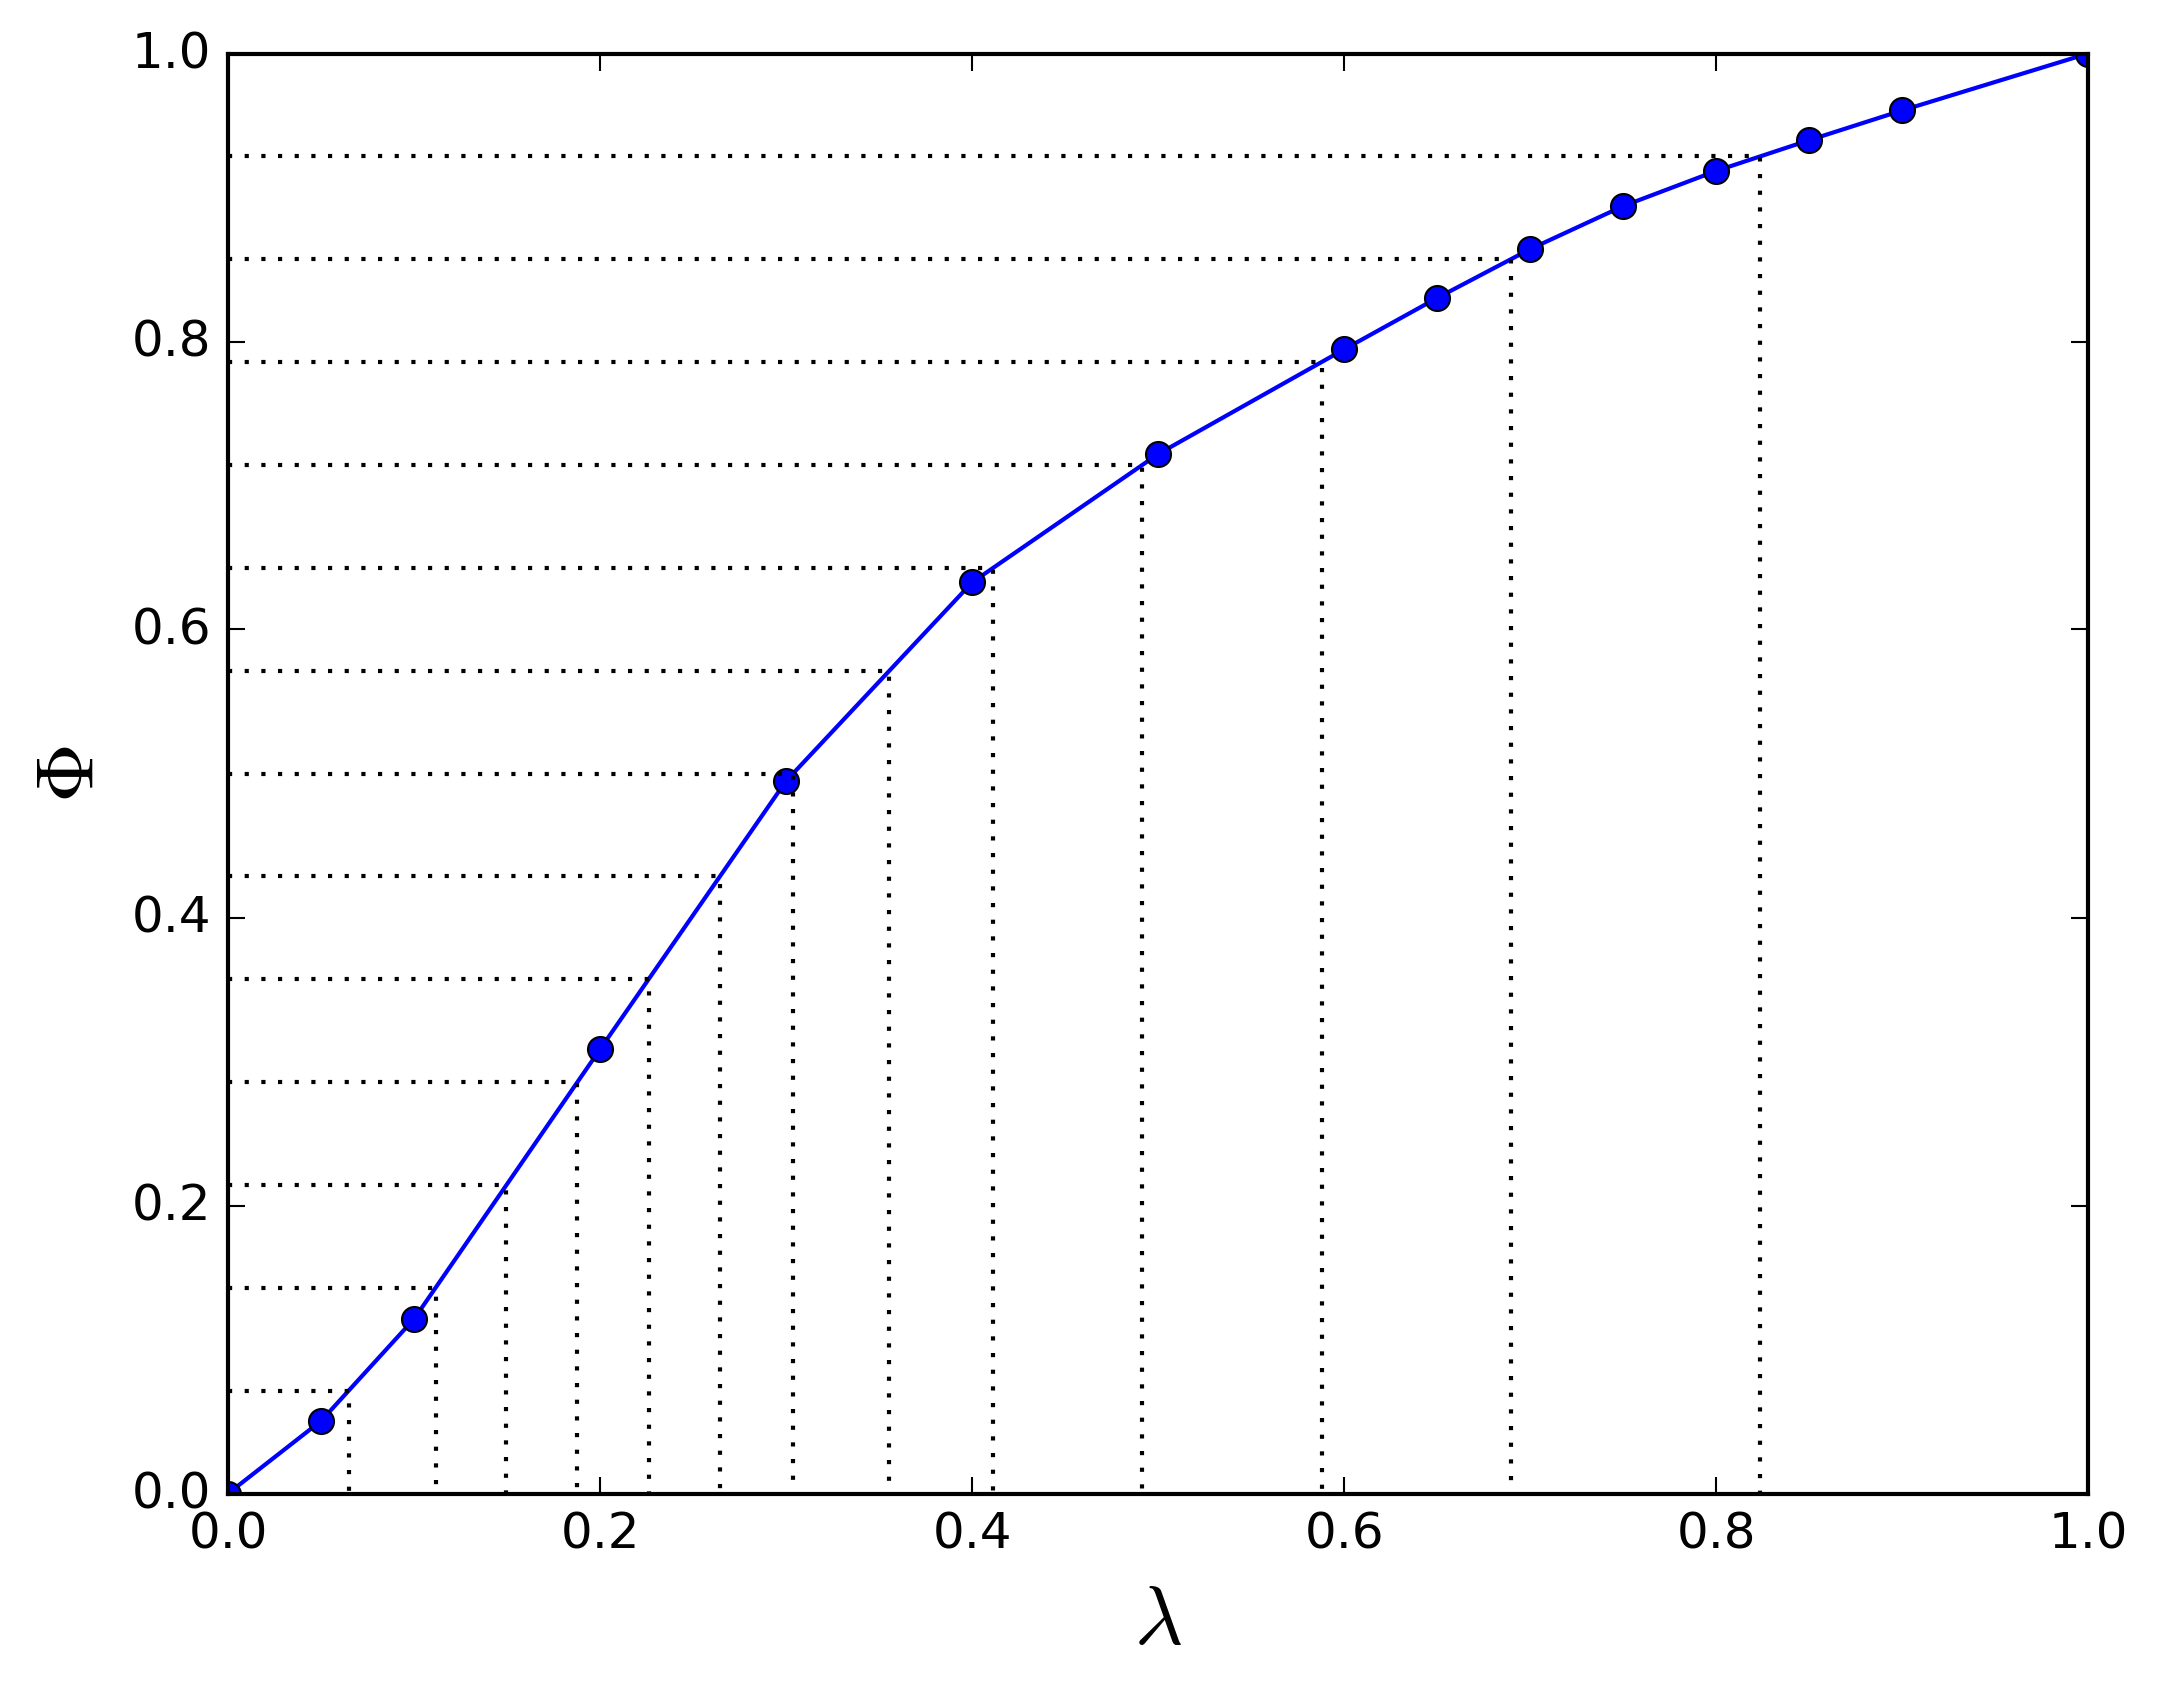
\includegraphics[width=0.8\linewidth]{Figures/optimized_cdf}
		\caption{Cumulative probability used to obtain the optimized values of $\lambda 's$ for the pair hexane+benzene.}
		\label{fig:optimized_cdf}
	\end{figure}
	
	\begin{table*}[h]
		\centering
		\caption{Calculated and experimental values for the solvation free energy differences (kcal/mol) of solutes in non-aqueous solvents.}
		\label{tbl:solv1}
		\begin{tabular}{cccccc}
			\hline\hline
			Solute       & Solvent   & $\Delta G_{solv}^{exp}$ & $\Delta G_{solv}^{Mie}$ & Absolute  &  \\
			&           &                         &                         & Deviation &  \\ \hline
			benzene      & hexane    & -3.96                   & -3.76  $\,$ $\pm$ 0.01       & 0.20      &  \\
			pyrene       & hexane    & -11.53                  & -10.82 $\pm$ 0.02       & 0.71      &  \\
			phenanthrene & hexane    & -10.01                  & -9.16  $\,$ $\pm$ 0.01       & 0.85      &  \\
			propane      & 1-octanol & -1.32                   & -1.36  $\,$ $\pm$ 0.03       & 0.04      &  \\
			anthracene   & 1-octanol & -11.72                  & -8.12   $\,$ $\pm$ 0.03       & 3.61      &  \\
			phenanthrene & 1-octanol & -10.22                  & -8.34  $\,$ $\pm$ 0.03       & 1.47      &  \\
			pyrene       & toluene   & -12.86                  & -11.74 $\pm$ 0.01       & 1.11      &  \\
			anthracene   & toluene   & -11.31                  & -9.90 $\,$ $\pm$ 0.01        & 1.41      &  \\ \hline\hline
			&
		\end{tabular}
	\end{table*}
	
	After the expanded ensemble simulations with the optimized intermediate states and weights, we calculated the solvation free energy differences with MBAR. The results obtained and the absolute deviations to experimental data \cite{doi:10.1021/ci034120c} are available  in Table \ref{tbl:solv1}. The numerical values for solvation free energies in hexane had overall smaller absolute deviations from experimental data than the deviations in the other solvents. Additionally, this force field presented better results for the pair hexane+benzene than the TraPPE force field (- 4.35  $\pm$ 0.05 kcal/mol) \cite{garrido2011} and the ELBA coarse-grained force field  (-2.92 $\pm$ 0.01 kcal/mol) \cite{doi:10.1021/acs.jctc.5b00963}. TraPPE is a force field parametrized with fluid-phase equilibria data that uses the Lennard-Jones potential to describe the non-bonded interactions. In the cited paper, they used the united-atom description of the TraPPE force field for the alkyl group, the all-atom description for the polar groups and the explicit-hydrogen approach for the aromatic groups. In the explicit-hydrogen approach, the interaction sites for all hydrogen atoms, some lone pair electrons, and bond centers are accounted for \cite{doi:10.1021/jp073586l}. In turn, the ELBA force field is a coarse-grained model that comprises six independent parameters. This force field models three carbons as one Lennard-Jones site and one water molecule as a single Lennard Jones site with a point dipole. We also present the solvation free energies corresponding to each alchemical state ($\lambda$) for all the pairs studied here in Figures \ref{fig:hex} to \ref{fig:tol}. Specifically observing the solvation free energy in hexane (Figure \ref{fig:hex}), we can see the effect of the molecule's size on the entropic region of the free energy curve. This region is corresponding to the first values of $\lambda$ where space in the solvent is being 'opened' for the insertion of the solute.
	
		\begin{figure}
			\centering
			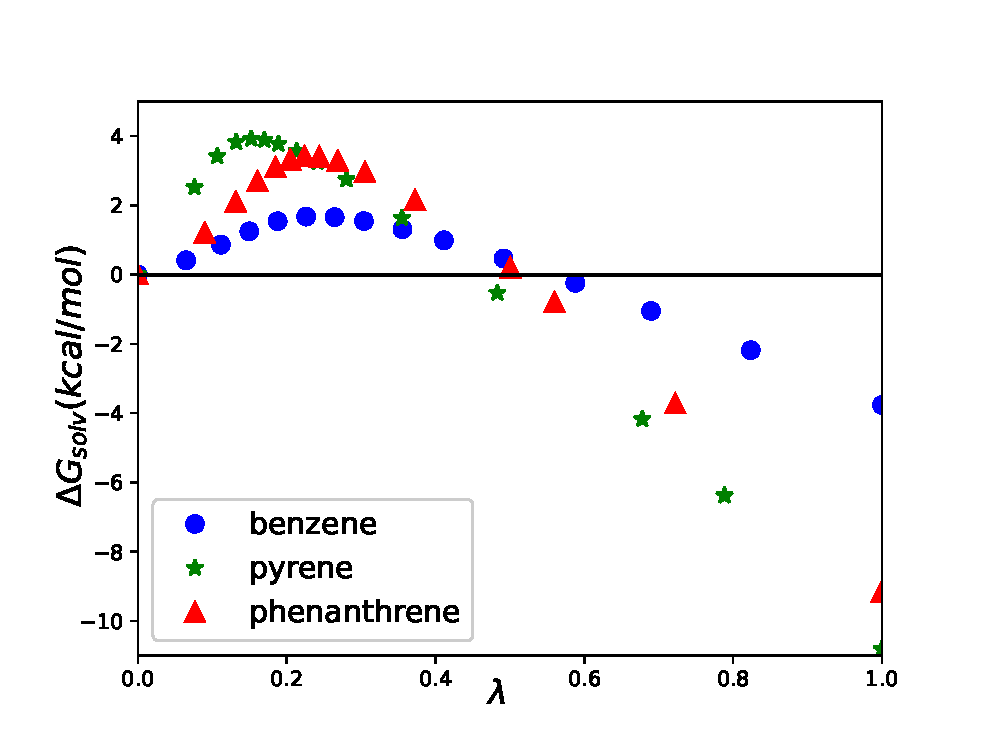
\includegraphics[width=1.0\linewidth]{Figures/hexart}
			\caption{Representation of solvation free energies of different solutes in hexane corresponding to each alchemical state.}
			\label{fig:hex}
		\end{figure}
		
		\begin{figure}
			\centering
			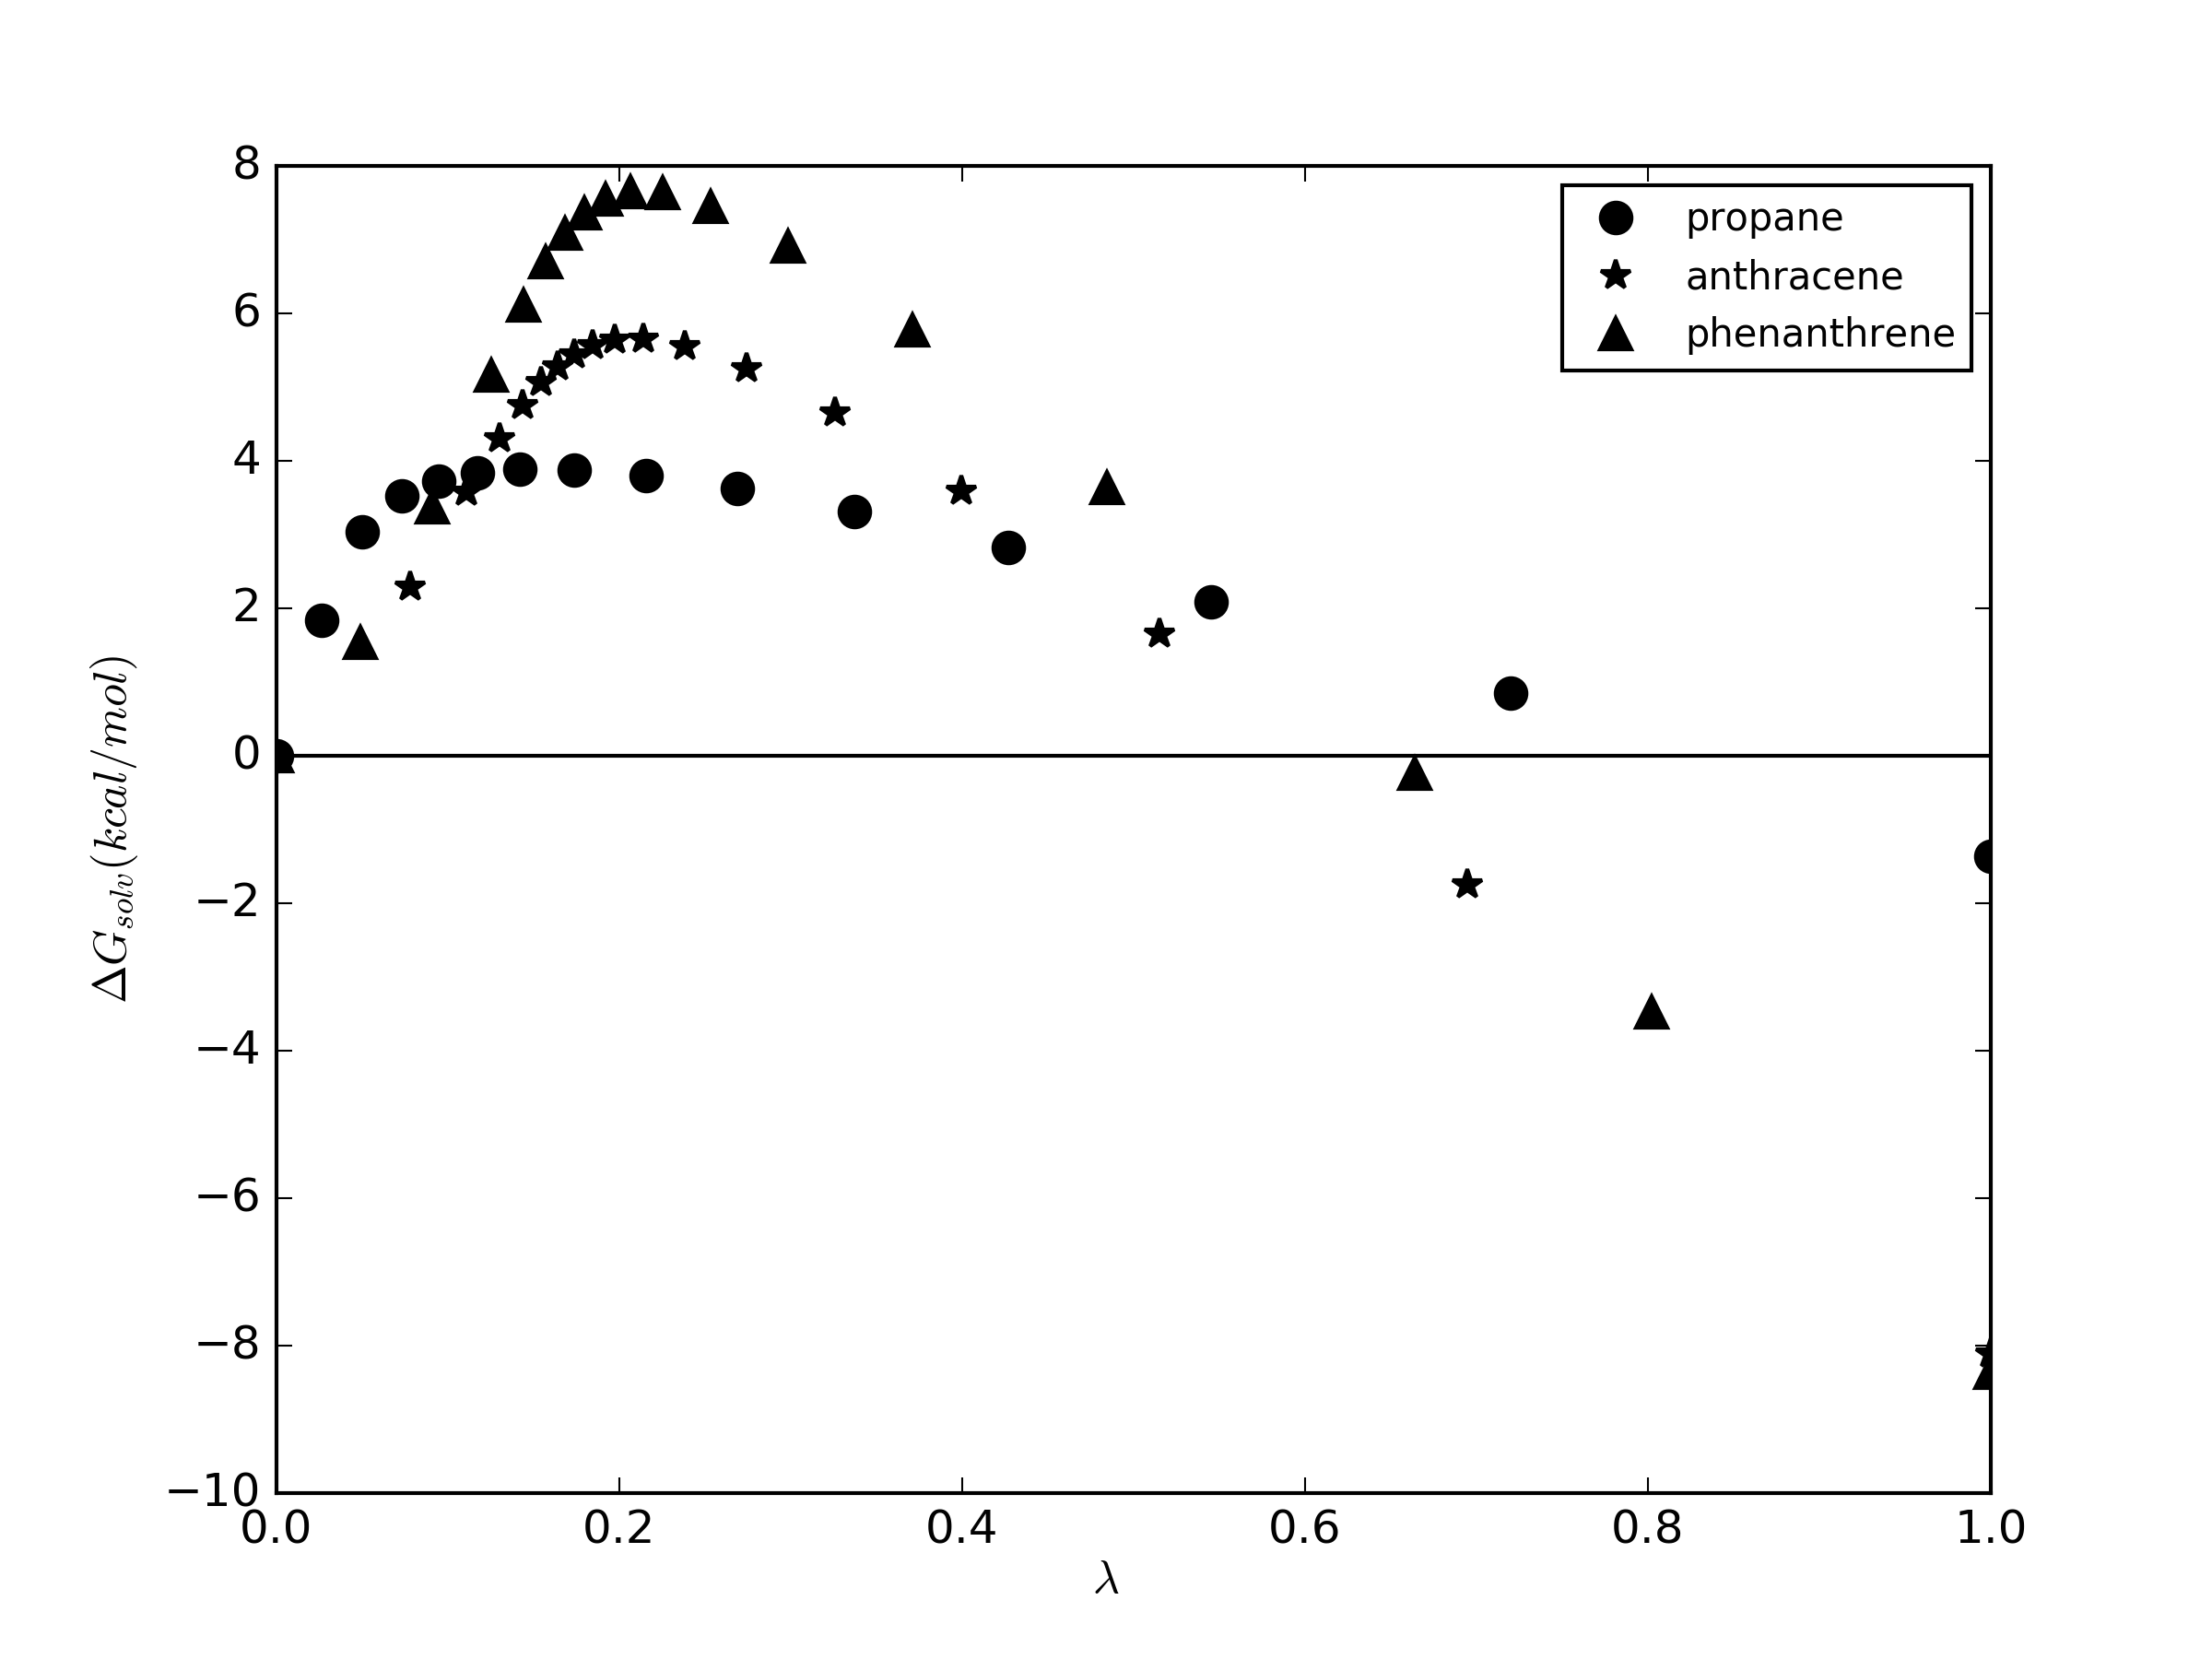
\includegraphics[width=1.0\linewidth]{Figures/octart}
			\caption{Representation of solvation free energies of different solutes in 1-octanol corresponding to each alchemical state.}
			\label{fig:oct}
		\end{figure}
		
		\begin{figure}
			\centering
			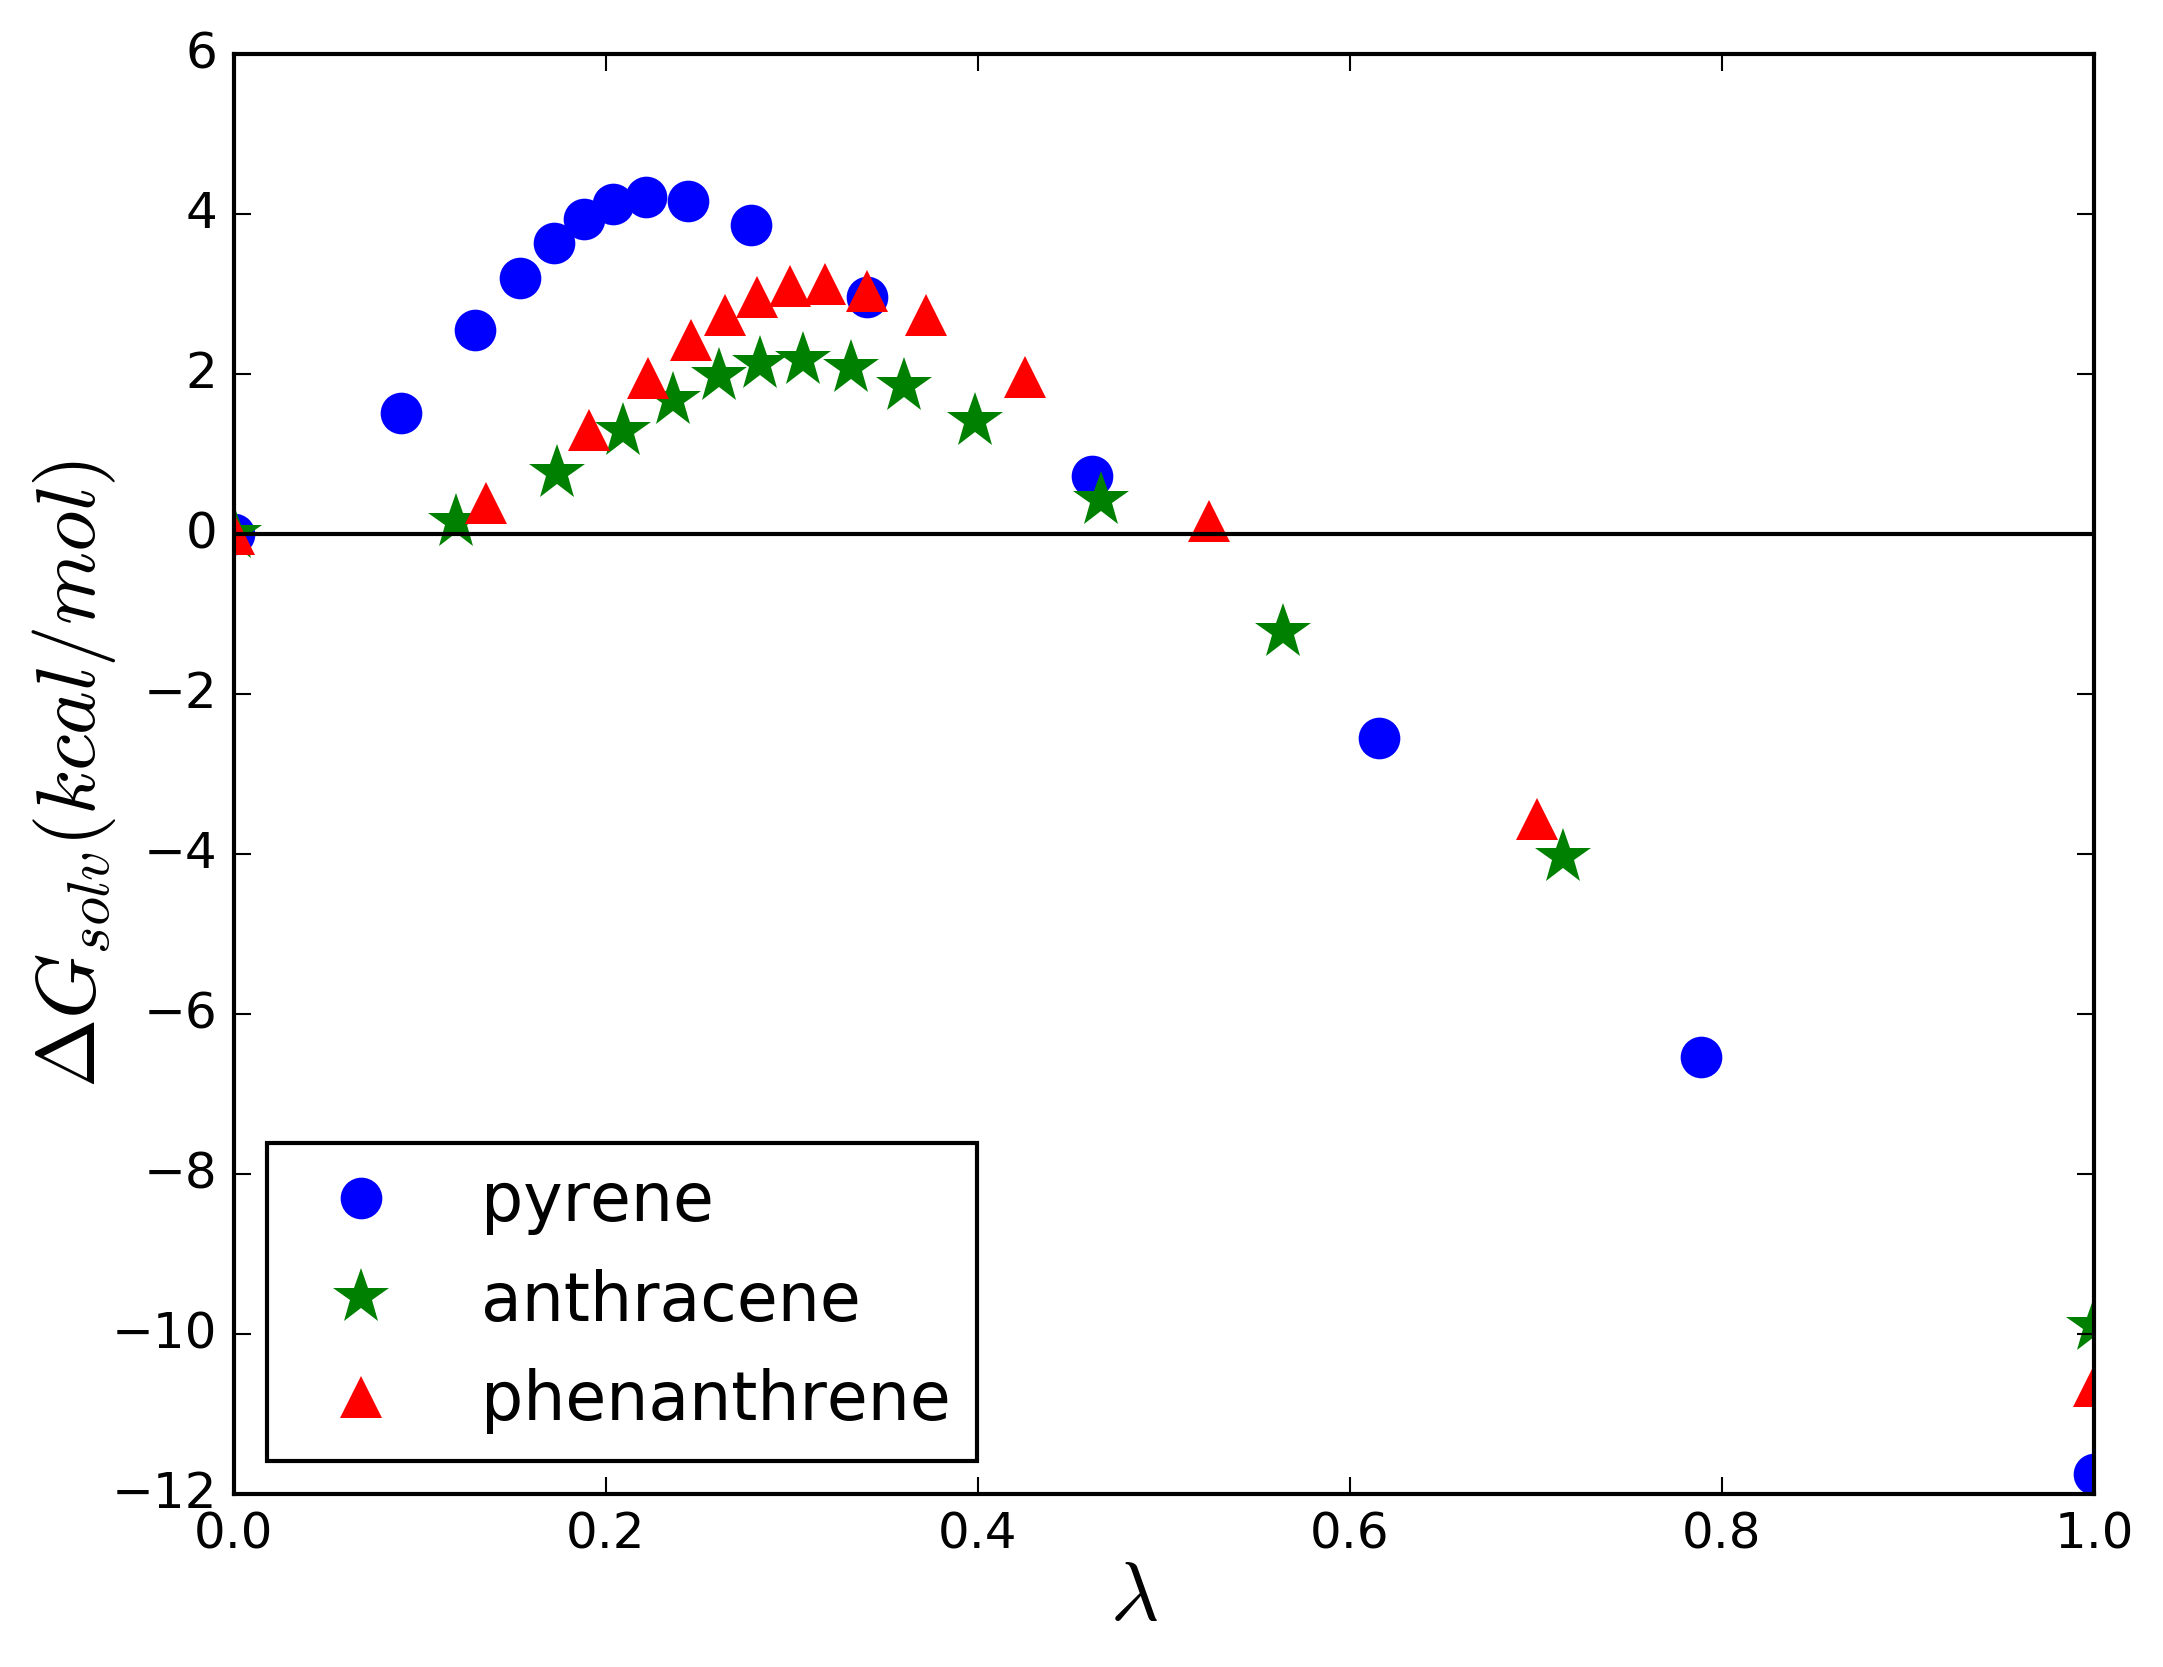
\includegraphics[width=1.0\linewidth]{Figures/tolart}
			\caption{Representation of solvation free energy profiles obtained with MD simulations of different solutes in toluene. }
			\label{fig:tol}
		\end{figure}
	
	We expected that a force field based on an EoS that does not explicitly account for hydrogen bond would not perform well for 1-octanol in mixtures since the parameterization of this molecule did not explicitly account for the interactions of association. All the beads representing 1-octanol have the same intermolecular parameter, and there is no distinction between the polar and apolar groups. Despite this, the solvation free energies of propane and phenanthrene in 1-octanol lied in the desired deviation range of 1-2 kcal/mol \cite{doimobley}. For propane, the observed deviation in solvation free energies was much smaller when compared to the other solutes, which can be attributed to the non polarity of propane and its smoother free energy curve, presented in Figure \ref{fig:oct}. Such solvation free energy of propane in 1-octanol also had a smaller deviation than the prediction of the ELBA force field (-0.92 $\pm$ 0.01) \cite{doi:10.1021/acs.jctc.5b00963}. The absolute deviation of the solvation free energy computed for anthracene in 1-octanol is much higher than the one calculated for phenanthrene in 1-octanol. The anthracene and phenanthrene molecules have the same geometry (Figure \ref{fig:fen5}) in the SAFT-$\gamma$ Mie model, although anthracene is a linear molecule and phenanthrene is not, and also similar physical properties. Hence, this high deviation of the solvation free energy of anthracene in 1-octanol may indicate a problem in the geometry chosen for anthracene in the SAFT-$\gamma$ Mie force field and the importance of the geometry in modeling the molecules with this force field.   
	
   The results also indicate a reasonable capability of the force field for predicting the solvation free energies of polyaromatic solutes in aromatic solvents. The influence of the molecular geometry on the solvation free energy curves was the same as the one observed for other solvents, as can be seen in Figure \ref{fig:tol}.  We also calculated the $\Delta G_{solv}$ for phenanthrene in pure toluene and in toluene+$CO_{2}$ mixtures. To the best of our knowledge, there are no available experimental data for these solvation free energies, but the previous results for phenanthrene in other solvents showed that the force field is adequate to describe the solvation phenomenon of phenanthrene in a pure aromatic solvent. Hence, we decided to carry out a qualitative study of the influence of $CO_{2}$ in the solvation free energies of phenanthrene in toluene in order to evaluate the description of this system with the SAFT-$\gamma$ Mie force field. The results for these sets are exposed in Table \ref{tbl:solvco2}. The increase of the mass fraction of $CO_{2}$ in toluene caused a small effect on the solvation free energies in the range of weight fractions (0.087-0.289) studied in this dissertation. First, the $\Delta G_{solv}$ decreased with the increase of $w_{CO_{2}}$ up to 0.119. After this, the effect was reversed, and carbon dioxide became an anti-solvent. Soroush et al. \cite{SOROUSH2014405} reported that asphaltene precipitation occurs when carbon dioxide mass fractions became higher than 0.10 in the system asphaltene+toluene+carbon dioxide, which is in agreement with the anti-solvent effect of carbon dioxide observed in the values calculated here. Although we noticed the anti-solvent effect, the differences observed are pretty small. These minor differences may indicate that the effect of $CO_{2}$ is negligible in the solvation of phenanthrene in toluene when using the SAFT-$\gamma$ Mie force field to model the molecules. Nevertheless, more studies need to be done to make a safe assertion about it. It is also worth remarking that this is a qualitative study due to the lack of experimental data. Overall, the methodology proposed by the SAFT-$\gamma$ Mie force field was satisfactory in predicting the solvation free energies of the pairs solvent-solute studied here. For the pair 1-octanol+anthracene, the performance obtained was not as good as it was for the other pairs. This result highlights the importance of choosing a correct geometry for this coarse-grained force field.    
	
	\begin{table}
		\centering
		\caption{Calculated values for the solvation free energy differences (kcal/mol) of phenanthrene in toluene+$CO_{2}$.}
		\label{tbl:solvco2}
		\begin{tabular}{ll}
			\hline\hline
			$w_{CO_{2}}$ & $\Delta G_{solv}^{Mie}$ \\ \hline
			0.0          & -10.65 $\pm$ 0.02       \\
			0.087        & -10.73 $\pm$ 0.02       \\
			0.119        & -10.78 $\pm$ 0.02       \\
			0.169        & -10.71 $\pm$ 0.02       \\
			0.289        & -10.69 $\pm$ 0.02       \\ \hline\hline
		\end{tabular}
	\end{table}
	
	\subsection{Hydration free energies}
	
Water is a solvent extensively used in experimental and computational studies. Because of this importance and the fact that water has unique properties, such as density maximum at 277 K and increased diffusivity upon compression, developing an accurate computational model for water is an ongoing quest \cite{hadley2012}. Hence, we also calculated the solvation free energies in water (hydration free energies) with the SAFT-$\gamma$ Mie force field. With these calculations, we intend to verify if this coarse-grained model would represent the water molecule correctly and would be a good alternative to decrease the computational cost of solvation studies with asphaltene models. The simulations with water as a solvent were carried out using widely studied solutes (propane, benzene) and polyaromatic solutes (toluene, phenanthrene) with a set of fifteen intermediate states.  We obtained these sets of $\lambda$ and $\eta$ with the same methodology used to acquire the sets for the solvation free energies with non-aqueous solvents, and they are exposed in Table \ref{tbl:lambdawater}, available in the Appendix. At first in our simulations, the binary interaction parameters of all aqueous mixtures were set to zero, but preliminary results for hydration free energies, displayed in Table \ref{tbl:solv2},  exhibited a high deviation from experimental data \cite{P29900000291, doi:10.1021/ct050097l}. With these results, the need for binary interaction parameters became clear. First, we estimated $k_{ij}$ with the SAFT-VR Mie EoS and experimental vapor pressure data, but this strategy also provided results that had high absolute deviations from the experimental data. Therefore, we used the approach of estimating $k_{ij}$ with the output from solvation free energy calculations with molecular dynamics, as described in the last paragraph of Section \ref{mds}.  We initially found individual values for the interaction parameter of each pair, but, since the parameters for aromatic solutes were very similar (0.148, 0.162, 0.152), we averaged these values. By doing that,  we obtained a general parameter for the water+aromatic pairs, which is exposed in Table \ref{tbl:kij}. Also in this table, we display the binary interaction parameter for the pair water+propane. 
	
	\begin{table}
		\centering
		\caption{Binary interaction parameters employed.}
		\label{tbl:kij}
		\begin{tabular}{cc}
			\hline\hline
			Pair              & $k_{ij}$ \\ \hline
			water+propane  & 0.067    \\
			water+aromatic & 0.154    \\ \hline\hline
		\end{tabular}
	\end{table}
	
	The relatively large $k_{ij}$ value of the interaction between aromatic solutes and water can be related to the lack of an explicit association term in the equation of state used to obtain the parameters for water. Actually, the SAFT-VR Mie has an association term \cite{lafitte2013}, but it was not incorporated in the force field. The SAFT-$\gamma$ Mie model for water \cite{lobanova2016} has two different temperature-dependent sets of parameters. The parameters utilized in this work were those estimated with experimental interfacial tension data. Hence, we tested the only binary interaction parameter for water+toluene estimated with MD interfacial data available in the literature \cite{herdes2017}. Nevertheless, the result also had a high absolute deviation, and this parameter could not be transferred to the calculation of the solvation free energy of toluene in water. 
	
	These issues faced by SAFT-$\gamma$ Mie model can also be related to the problems of modeling water with a coarse-grained force field. One of the main difficulties is the choice of which water molecules are going to be represented by which specific beads since water molecules move independently and are only bound by non-bonded interactions \cite{hadley2010,hadley2012}. The  SAFT-$\gamma$ Mie water considers that one water molecule corresponds to one bead. This strategy only saves a small amount of simulation time, but it can predict properties at physiological temperatures unlike other more aggressive models such as the MARTINI, which considers that one bead represents various water molecules. In light of all these problems related to modeling the water molecule, the SAFT-$\gamma$ Mie force field appears to be a good alternative when working close to room temperatures, but the necessity of additional parameters estimated with molecular simulation indicates severe flaws in the methodology. This estimation of the binary parameter increased significantly the simulation time required to calculate the hydration free energies, since we had to carry out three additional simulations for every pair water-solute and then three additional simulations for the three water+polyaromatic solutes in order to test the averaged binary interaction parameter. If these simulations are necessary for every time a new mixture with water is going to be studied with the SAFT-$\gamma$ Mie force field, the use of this model can become impractical.  With this idea in mind, a useful investigation to be made is to check how much other pairs of water+aromatic solute can be modeled using the binary interaction parameter estimated here. Using these binary interaction parameters calculated with data from molecular dynamics, we then obtained the final hydration free energies presented in Table \ref{tbl:solv2}. 
	
	\begin{table*}
		\centering
		\caption{Calculated and experimental hydration free energy differences  (kcal/mol) of solutes in water.}
		\label{tbl:solv2}
		\begin{tabular}{cccccc}
			\hline\hline
			Solute       & $\Delta G_{solv}^{exp}$ & \vtop{\hbox{\strut $\Delta G_{solv}^{Mie}$}\hbox{\strut $k_{ij} = 0$}} & \vtop{\hbox{\strut Absolute}\hbox{\strut Deviation}} & \vtop{\hbox{\strut $\Delta G_{solv}^{Mie}$}\hbox{\strut $k_{ij} \neq 0$}} & \vtop{\hbox{\strut Absolute}\hbox{\strut Deviation}} \\ \hline
			propane      & 2.00 $\pm$ 0.20         & 1.10 $\pm$ 0.01                                                        & 0.90                                                 & 2.01 $\pm$ 0.01                                                           & 0.01                                                 \\
			benzene      & -0.86 $\pm$ 0.20        & -4.45 $\pm$ 0.03                                                       & 3.59                                                 & -1.12 $\pm$ 0.01                                                          & 0.26                                                 \\
			toluene      & -0.83 $\pm$ 0.20        & -10.98 $\pm$ 0.30                                                      & 10.15                                                & -0.84 $\pm$ 0.01                                                          & 0.01                                                 \\
			phenanthrene & -3.88 $\pm$ 0.60        & -10.90 $\pm$ 0.04                                                      & 7.12                                                 & -3.47 $\pm$ 0.02                                                          & 0.41                                                 \\ \hline\hline
			%    RMSE    &                         &                                                                        & 0.24                                                 &  \\
			%    \hline  &                         &
		\end{tabular}
		
	\end{table*}
	
Hydration free energies calculated using the SAFT-$\gamma$ Mie force field with $k_{ij} \neq 0$ had low absolute deviations from the experimental data, as expected since the parameters were adjusted to fit these experimental data. Hydration free energies have also been calculated for the pairs studied here by Genheden \cite{doi:10.1021/acs.jctc.5b00963} with the ELBA force field and by Mobley and Guthrie \cite{PMID:24928188} with the GAFF force field for the solutes and with the TIP3P model for water. The GAFF (General Amber Force Field) force field is an all-atom model that consists of bonded and non-bonded parameters and is suitable for the study of a significant number of molecules. In turn, the TIP3P model considers that water is a rigid monomer represented by three interacting sites with non-bonded interactions and Coulombic interactions \cite{doi:10.1063/1.445869}. Both the GAFF and the TIP3P models use the Lennard-Jones potential to calculate the non-bonded interactions.

Comparing the three aforementioned force fields, the root mean square error (RMSE) of all the pairs tested with the SAFT-$\gamma$ Mie model was  0.24, the RMSE for hydration free energies obtained with the GAFF force field was 0.73, and that for the ELBA coarse-grained force field was 0.44. The difference in between the results of GAFF (-5.26$\pm$0.03) and SAFT-$\gamma$ Mie (-3.47 $\pm$ 0.02) force fields is significantly high for phenanthrene, hence the coarse-grained force field with a binary parameter is preferred if the application requires a high level of accuracy. The results also indicated that the SAFT-$\gamma$ Mie model with the binary interaction parameter performed better than the ELBA force field in modeling the solvation phenomenon of the pairs studied in this work, but performed worse with the binary parameter set to zero. This difference in performance occurred despite the fact that both the SAFT-$\gamma$ Mie and ELBA models have the same level of coarse-graining for the solvent (one bead represents one water molecule). Therefore, the choice between the two coarse-grained models is dependent on the availability and transferability of binary interaction parameters of the Mie Model. We also present, for the SAFT-$\gamma$ Mie force field, the hydration free energy profiles in Figure \ref{fig:water}. Bigger molecules had steeper free energy profiles, as it was for the solvation free energy study in other solvents. We also observe that the hydration free energy for the first non-zero $\lambda$ is negative for benzene and toluene when a positive value is expected since free energy is required to 'open space' in the solvent for the solute's insertion. This anomaly can be caused by the fact that the attractive term in the Mie potential compensates the need to open space. 
	
	\begin{figure}
		\centering
		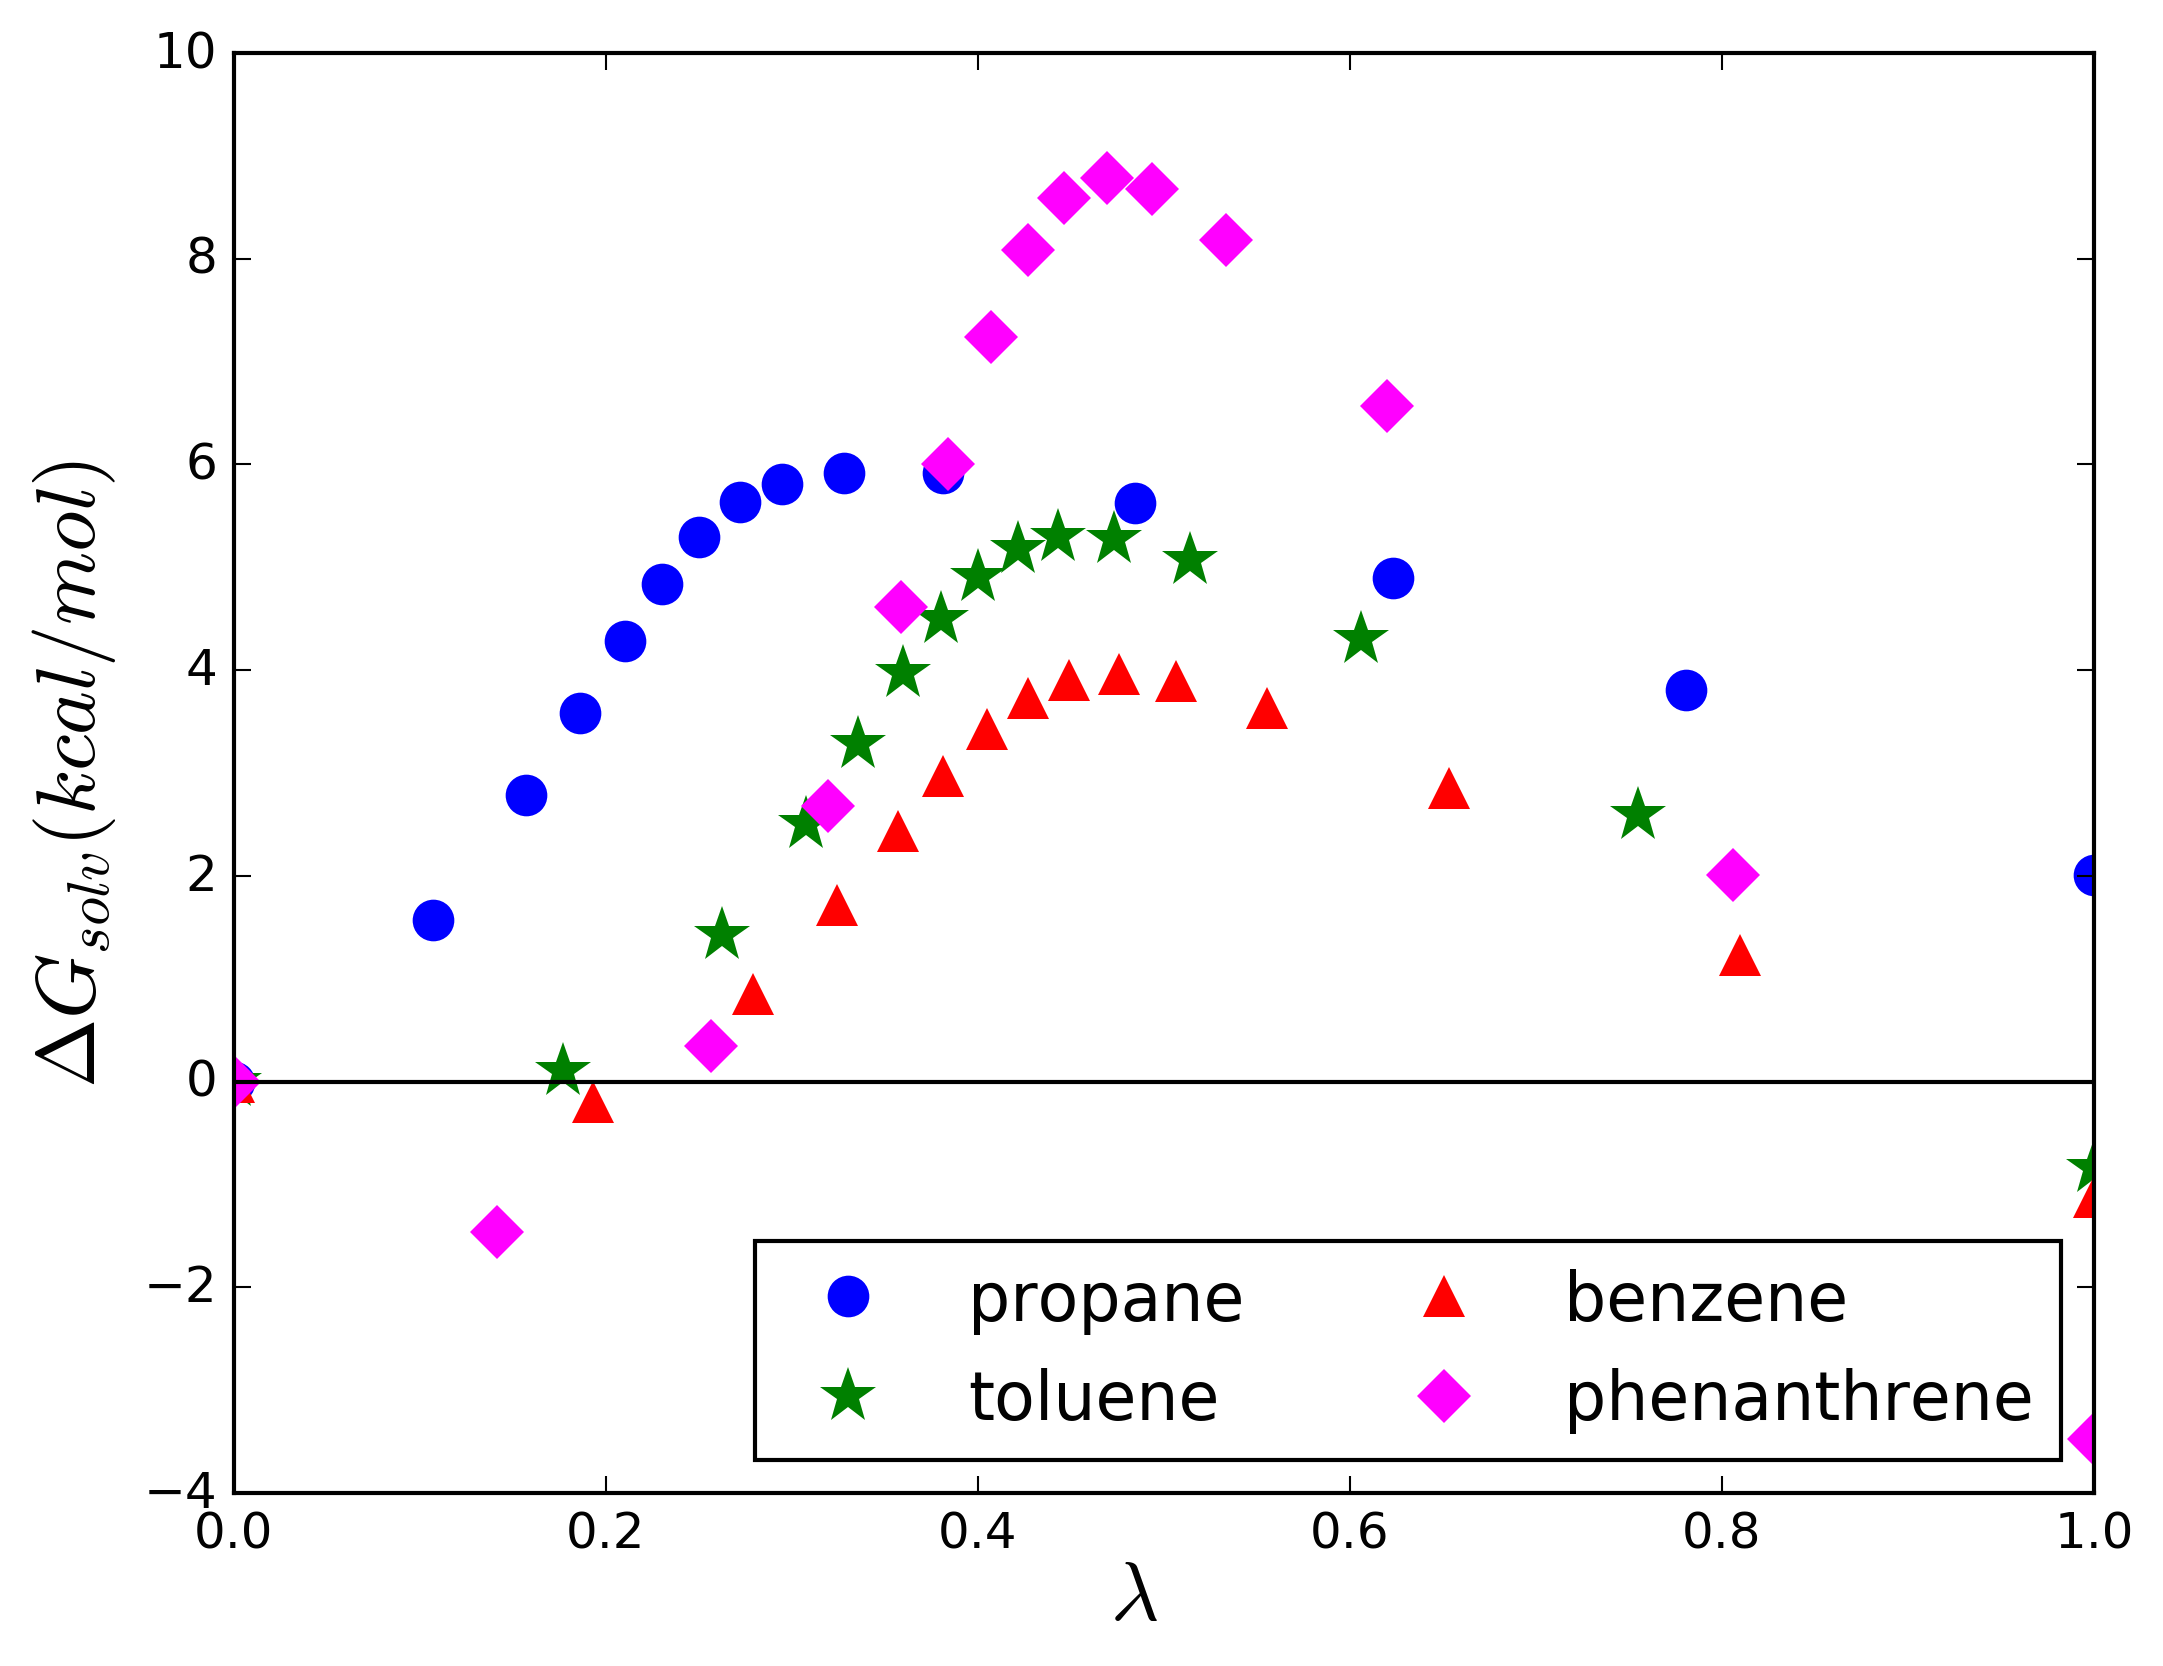
\includegraphics[width=1.0\linewidth]{Figures/waterart}
	\caption{Representation of hydration free energies of different solutes corresponding to each alchemical state.}
	\label{fig:water}
    \end{figure}

The results found here for both the solvation free energies and hydration free energies fulfilled the intentions of this dissertation. We assessed the prediction capability of the SAFT-$\gamma$ Mie force field and provided satisfactory solvation free energy estimates of PAHs using a coarse-grained force field. In addition to that, we found flaws in the methodology used by the SAFT-$\gamma$ Mie force field to model the water molecule. Hence, these shortcomings of this model can now be addressed, and the force field can even be improved by using other mixing rules to avoid the use of a binary parameter or, even, using hydration free energy estimates in the parameterization of water. These results also encourage us to calculate solvation free energies of more complex molecules mimicking asphaltenes in non-aqueous solvents in future studies.  
	
	\section{Conclusions}
This study consisted in the study of solvation free energy calculations of aromatic solutes in different solvents by using the SAFT-$\gamma$ Mie coarse-grained force field. Solvation free energy studies are mostly done using water as a solvent and with all-atom force fields based on the Lennard-Jones potential. Therefore, with this study, we were able to provide data about the capability of a coarse-grained force field based on the Mie potential in calculating solvation free energies. Additionally, the solvation free energy estimations carried out here can help improve the SAFT-$\gamma$  Mie force field since these calculations are helpful in identifying errors and shortcomings in the modeling process. The SAFT-$\gamma$ Mie uses the SAFT-VR Mie EoS in its parameterization, which results in a relatively straightforward top-down method of obtaining parameters. Following this strategy, the phenanthrene parameters, which were not available in the original database of this force field, were obtained using vapor-liquid equilibrium data.

To perform our expanded ensemble simulations, we optimized the coupling parameters and their respective simulation weights. The resulting potential energies from the expanded ensemble simulations then served as input to estimate solvation free energy differences with the MBAR method. The results for non-aqueous solvents had absolute deviations from the experimental
data of less than 2.0 kcal/mol, except for the pair 1-octanol+anthracene. We also observed the geometry effect on the free energy curves - larger molecules had steeper curves and more substantial absolute deviations. The influence of carbon dioxide on the solvation free energy of phenanthrene in toluene was found to be negligible according to the SAFT-$\gamma$ Mie force field. Hydration free energy calculations with the SAFT-$\gamma$ Mie model required the use of relatively large values of $k_{ij}$ to produce satisfactory results. We chose to estimate the parameter with the output from molecular dynamics data since the strategy of using the SAFT-VR Mie EoS provided high absolute deviations from the experimental data. This necessity of one additional parameter probably happens due to the lack of a term to account for the hydrogen bond in the EoS on which this force field is based and due to problems associated with the coarse-graining of water molecules. The results obtained with $k_{ij}$ estimated with MD output were satisfactory, the absolute deviations from the experimental data found were smaller than the ones for the GAFF and ELBA force fields.

Overall, the SAFT-$\gamma$ Mie force field proved to be a suitable model to represent the solvation phenomenon of non-aqueous solvents. It correctly described solvation free energies of solutes mimicking asphaltenes dissolved in hexane, toluene, 1-octanol. However, the calculation of hydration free energies required the use of a binary interaction parameter estimated with MD output, which increased the simulation time significantly. This fact evidenced flaws in the methodology used by the SAFT-$\gamma$ force field and raised questions about the feasibility of this model for hydration free energy calculations. Nevertheless, the SAFT-$\gamma$ Mie force field for water used here does not predict freezing at room temperature as other force fields do, which is essential for our hydration free energy calculations. Therefore, it would be relevant to test if the binary interaction parameter for our aromatic solutes estimated here can be used in hydration free energy calculations of other aromatic solutes and if we could use MBAR to obtain the $k_{ij}$ through reweighting. Hence, we would only need to carry out molecular dynamics simulations with one value of $k_{ij}$, and then use this output to estimate with MBAR the results with other $k_{ij} 's $. We also have some ideas that could be developed in the future using the results from this dissertation. The SAFT-$\gamma$ Mie force field could be used to model larger asphaltene models and, consequently, increase the scale of the simulations we performed. Additionally, it would be a valid investigation to study new methodologies to calculate solubility with solvation free energies using the SAFT-$\gamma$ Mie force field.



	
	\section{Acknowledgement}
	
	The authors thank the financial support provided by Cenpes/Petrobras (project code: 17.564). 
	
	\section*{References}
	
	\bibliography{mybibfile}
    	
	\appendix
	\section{}
	\label{}
\begin{table}[h]
	\centering
	\caption{Optimized values of $\lambda $ and $\eta $ for the hexane+solute pairs.}
	\label{tbl:lambdahex}
	\begin{tabular}{cccccc}
		\hline\hline
		\multicolumn{2}{c}{benzene}&\multicolumn{2}{c}{pyrene}& \multicolumn{2}{c}{phenanthrene}\\
		\hline\hline
		$\lambda$ & $\eta$& $\lambda$ & $\eta$  & $\lambda$ & $\eta$   \\ 
		\hline\hline
		0.000     &0.000      & 0.000    &    0.000    &    0.000    &    0.000    \\
		0.065     &0.708  & 0.076    &    4.234    &    0.090    &    1.981    \\
		0.112     &1.385  & 0.107    &    5.620    &    0.132    &    3.461    \\
		0.15      &1.892  & 0.132    &    6.499    &    0.161    &    4.494    \\
		0.188     &2.399  & 0.152    &    6.690    &    0.185    &    5.185    \\
		0.226     &2.519  & 0.170    &    6.643    &    0.205    &    5.552    \\
		0.264     &2.457  & 0.189    &    6.461    &    0.224    &    5.725    \\
		0.304     &2.367  & 0.213    &    6.091    &    0.244    &    5.722    \\
		0.356     &1.921  & 0.242    &    5.566    &    0.268    &    5.523    \\
		0.411     &1.411  & 0.280    &    4.729    &    0.305    &    4.975    \\
		0.492     &0.524  & 0.355    &    2.853    &    0.372    &    3.576    \\
		0.588     &-0.663 & 0.483    &    -0.778    &    0.500    &    0.297    \\
		0.69      &-2.016 & 0.678    &    -6.947    &    0.560    &    -1.390    \\
		0.824     &-3.922 & 0.788    &    -10.631    &    0.722    &    -6.309    \\
		1.000         &-6.583  &1.000      &    -18.141    &    1.000    &    -15.448    \\
		\hline\hline   
	\end{tabular}
\end{table}
\begin{table*}[h]
	\centering
	\caption{Optimized values of $\lambda $ and $\eta$ for the 1-octanol+solute pairs.}
	\begin{tabular}{cccccc}
		\hline\hline
		\multicolumn{2}{c}{propane}& \multicolumn{2}{c}{anthracene}& \multicolumn{2}{c}{phenanthrene}\\
		\hline\hline
		$\lambda$ & $\eta$ & $\lambda$ & $\eta$  & $\lambda$ & $\eta$   \\ 
		\hline\hline
		0.000    &    0.000    &    0.000    &    0.000    &    0.000    &    0.000    \\
		0.027    &    3.126    &    0.078    &    3.932    &    0.049    &    2.578    \\
		0.050    &    5.109    &    0.111    &    6.178    &    0.091    &    5.663    \\
		0.073    &    6.093    &    0.130    &    7.426    &    0.125    &    8.575    \\
		0.095    &    6.570    &    0.143    &    8.201    &    0.144    &    10.069    \\
		0.117    &    6.826    &    0.154    &    8.717    &    0.157    &    10.978    \\
		0.142    &    6.956    &    0.164    &    9.085    &    0.169    &    11.599    \\
		0.174    &    6.969    &    0.174    &    9.357    &    0.180    &    12.040    \\
		0.215    &    6.847    &    0.184    &    9.556    &    0.192    &    12.340    \\
		0.269    &    6.554    &    0.197    &    9.676    &    0.206    &    12.499    \\
		0.337    &    6.050    &    0.214    &    9.681    &    0.225    &    12.478    \\
		0.427    &    5.228    &    0.238    &    9.490    &    0.253    &    12.161    \\
		0.545    &    3.955    &    0.274    &    8.958    &    0.298    &    11.280    \\
		0.720    &    1.843    &    0.326    &    7.906    &    0.371    &    9.406    \\
		1.000    &    -1.903    &    0.399    &    6.088    &    0.484    &    5.891    \\
		&        &    0.515    &    2.777    &    0.664    &    -0.516    \\
		&        &    0.695    &    -2.960    &    0.802    &    -5.908    \\
		&        &    1.000    &    -13.768    &    1.000    &    -14.073    \\
		\hline\hline
	\end{tabular}
\end{table*}
\begin{table*}[h]
	\centering
	\caption{Optimized values of $\lambda $ and $\eta$ for the toluene+solute pairs.}
	\begin{tabular}{cccccc}
		\hline\hline
		\multicolumn{2}{c}{pyrene}& \multicolumn{2}{c}{anthracene}& \multicolumn{2}{c}{phenanthrene}\\
		\hline\hline
		$\lambda$ & $\eta$ & $\lambda$ & $\eta$  & $\lambda$ & $\eta$   \\ 
		\hline\hline
		0.000    &    0.000    &    0.000    &    0.000    &    0.000    &    0.000    \\
		0.090    &    2.563    &    0.119    &    0.218    &    0.136    &    0.726    \\
		0.130    &    4.338    &    0.174    &    1.210    &    0.191    &    2.307    \\
		0.154    &    5.439    &    0.209    &    2.052    &    0.223    &    3.430    \\
		0.172    &    6.181    &    0.236    &    2.664    &    0.246    &    4.233    \\
		0.188    &    6.670    &    0.261    &    3.122    &    0.264    &    4.780    \\
		0.204    &    6.986    &    0.283    &    3.378    &    0.281    &    5.149    \\
		0.222    &    7.121    &    0.306    &    3.449    &    0.299    &    5.354    \\
		0.244    &    7.025    &    0.332    &    3.311    &    0.318    &    5.389    \\
		0.278    &    6.520    &    0.360    &    2.936    &    0.340    &    5.222    \\
		0.340    &    5.010    &    0.399    &    2.209    &    0.372    &    4.717    \\
		0.462    &    1.247    &    0.466    &    0.567    &    0.425    &    3.440    \\
		0.616    &    -4.283    &    0.564    &    -2.211    &    0.524    &    0.444    \\
		0.788    &    -11.032    &    0.715    &    -6.983    &    0.701    &    -5.814    \\
		1.000    &    -19.814    &    1.000    &    -16.923    &    1.000    &    -17.803    \\        
		\hline\hline
	\end{tabular}
\end{table*}

\begin{table*}[h]
	\centering
	\caption{Optimized values of $\lambda $ and $\eta $ for the phenanthrene+$CO_{2}$+ toluene mixture with different values of $w_{CO_{2}}$.}
	\label{tbl:lambdaco2}
	\begin{tabular}{cccccccc}
		\hline\hline
		\multicolumn{2}{c}{$w_{CO_{2}}=0.087$}& \multicolumn{2}{c}{$w_{CO_{2}}=0.119$}& \multicolumn{2}{c}{$w_{CO_{2}}=0.169$}& \multicolumn{2}{c}{$w_{CO_{2}}=0.289$}\\
		\hline\hline
		$\lambda$ & $\eta$ & $\lambda$ & $\eta$  & $\lambda$ & $\eta$  & $\lambda$ & $\eta$ \\ 
		\hline\hline
		0.000    &    0.000    &    0.000    &    0.000    &    0.000    &    0.000    &    0.000    &    0.000    \\
		0.128    &    0.604    &    0.128    &    0.732    &    0.064    &    0.883    &    0.066    &    0.806    \\
		0.184    &    2.067    &    0.186    &    2.223    &    0.108    &    0.764    &    0.111    &    0.760    \\
		0.217    &    3.164    &    0.219    &    3.319    &    0.175    &    1.969    &    0.172    &    1.983    \\
		0.240    &    3.940    &    0.244    &    4.098    &    0.214    &    3.156    &    0.204    &    2.967    \\
		0.260    &    4.472    &    0.267    &    4.704    &    0.240    &    3.974    &    0.227    &    3.627    \\
		0.277    &    4.823    &    0.289    &    5.031    &    0.258    &    4.457    &    0.245    &    4.082    \\
		0.295    &    5.035    &    0.313    &    5.084    &    0.273    &    4.750    &    0.262    &    4.395    \\
		0.318    &    5.059    &    0.339    &    4.950    &    0.287    &    4.921    &    0.279    &    4.583    \\
		0.347    &    4.762    &    0.373    &    4.371    &    0.305    &    4.962    &    0.299    &    4.621    \\
		0.397    &    3.753    &    0.425    &    3.055    &    0.326    &    4.885    &    0.325    &    4.423    \\
		0.491    &    1.031    &    0.488    &    1.196    &    0.361    &    4.401    &    0.365    &    3.739    \\
		0.670    &    -5.148    &    0.525    &    -0.027    &    0.419    &    2.990    &    0.428    &    2.198    \\
		0.791    &    -9.713    &    0.730    &    -7.185    &    0.527    &    -0.299    &    0.530    &    -0.842    \\
		1.000    &    -18.098    &    1.000    &    -17.769    &    0.697    &    -6.180    &    0.701    &    -6.763    \\
		&        &        &        &    1.000    &    -17.998    &    1.000    &    -18.163    \\
		\hline\hline
	\end{tabular}
\end{table*}

\begin{table*}[h]
	\centering
	\caption{Optimized values of $\lambda $ and $\eta $ for the water+solute pairs. }
	\label{tbl:lambdawater}
	\begin{tabular}{cccccccc}
		\hline\hline
		\multicolumn{2}{c}{propane}& \multicolumn{2}{c}{benzene}& \multicolumn{2}{c}{toluene}& \multicolumn{2}{c}{phenanthrene}\\
		\hline\hline
		$\lambda$ & $\eta$ & $\lambda$ & $\eta$  & $\lambda$ & $\eta$  & $\lambda$ & $\eta$ \\ 
		\hline\hline
		0.000    &    0.000    &    0.000    &    0.000    &    0.000    &    0.000    &    0.000    &    0.000    \\
		0.107    &    2.673    &    0.193    &    -0.295    &    0.177    &    0.182    &    0.142    &    -2.462    \\
		0.157    &    4.703    &    0.279    &    1.468    &    0.262    &    2.432    &    0.256    &    0.597    \\
		0.186    &    6.047    &    0.324    &    2.931    &    0.307    &    4.244    &    0.319    &    4.504    \\
		0.210    &    7.148    &    0.357    &    4.168    &    0.336    &    5.552    &    0.358    &    7.762    \\
		0.230    &    8.017    &    0.381    &    5.091    &    0.360    &    6.696    &    0.384    &    10.104    \\
		0.250    &    8.883    &    0.405    &    5.891    &    0.380    &    7.558    &    0.407    &    12.185    \\
		0.272    &    9.291    &    0.427    &    6.443    &    0.400    &    8.233    &    0.427    &    13.607    \\
		0.294    &    9.700    &    0.449    &    6.770    &    0.422    &    8.678    &    0.446    &    14.490    \\
		0.328    &    9.900    &    0.476    &    6.900    &    0.443    &    8.859    &    0.469    &    14.834    \\
		0.381    &    9.930    &    0.506    &    6.805    &    0.473    &    8.810    &    0.494    &    14.667    \\
		0.484    &    9.463    &    0.555    &    6.392    &    0.514    &    8.452    &    0.533    &    13.832    \\
		0.623    &    8.195    &    0.653    &    5.109    &    0.606    &    7.148    &    0.620    &    11.069    \\
		0.781    &    6.378    &    0.810    &    2.421    &    0.755    &    4.273    &    0.806    &    3.279    \\
		1.000    &    3.333    &    1.000    &    -1.480    &    1.000    &    -1.547    &    1.000    &    -6.122    \\        
		\hline\hline
	\end{tabular}
\end{table*}
\end{document}